\chapter{\MakeUppercase{Передумови та особливості використання активного ультразвуку}}



\section{Ефекти впливу ультразвуку на мікроелектронні структури та \\ матеріали \label{Oglyad}}
%\chapter{\MakeUppercase{Передумови та перспективи використання активного ультразвуку в мікроелектроніці}\label{Oglyad}}

Загальновідомо, що поширення акустичних хвиль (АХ) у кристалічних тілах пов'язане з вимушеним коливальним рухом атомів.
Явища, які супроводжують подібні процеси, знаходять своє застосування у багатьох прикладних сферах, включаючи і мікроелектроніку.
В останньому випадку найяскравішим прикладом є акустоелектроніка --- галузь, що базується на використанні взаємодії акустичних та електричних сигналів у п'єзоелектричних середовищах.
%Загалом явища, пов'язані з механічними коливаннями пружного середовища, широко застосовуються у мікроелектроніці.
%В Це стосується, насамперед акустоелектроніки --- галузі, що базується на використанні взаємодії акустичних та електричних сигналів у п'єзоелектричних середовищах.
%Існує величезна кількість різноманітних акустоелектричних фільтрів, ліній затримки, трансформаторів та інших пристроїв,
%принцип роботи яких базується на використанні п'єзоелектричного ефекту.
Проте у цьому підрозділі класичний ефект акустоелектронної взаємодії у об'ємних кристалах залишиться поза увагою і буде
розглянуто, переважно, дещо інший аспект використання ультразвуку,
зумовлений, насамперед, можливістю акусто--індукованої (АІ) перебудови дефектної підсистеми напівпровідників.

Дефекти, як відомо, є визначальними для властивостей як самих кристалів, так і приладів на їхній основі.
У літературі вже достатньо давно використовується термін
<<інженерія дефектів>>, який передбачає нерівноважну модифікацію дефектно--домішкової підсистеми з метою отримання нових властистовостей кристала, структури чи приладу шляхом формування <<потрібних>> активних центрів чи нанокластерів \cite{Smirnov}.
%Проте цей класичний ефект акустоелектронної взаємодії у об'ємних кристалах ми залишимо поза увагою, і в цьому розділі
%розглянемо,переважно, дещо інший аспект використання акустичних хвиль (АХ),
%зумовлений, насамперед, можливістю акустоіндукованих (АІ) процесів перебудови дефектної підсистеми напівпровідників, яка, як відомо, є визначальною для властивостей як самих кристалів, так і приладів на їх основі.
Безумовно, найбільш поширені та вивчені методи цього технологічного напряму пов'язані з
\begin{enumerate}[label=\asbuk*),leftmargin=0em,itemindent=1.5em]
\item використанням висотемпературних обробок (відпалів), різноманітних за тривалістю, атмосферою та іншими умовами проведення;
\item опромінення частинками різної природи (високоенергетичними фотонами, електронами, нейтронами, іонами) та енергії;
\item вибором режиму (температури, швидкості, атомарного складу сировини тощо) вирощування кристалу.
\end{enumerate}
%а)~використанням висотемпературних обробок (відпалів), різноманітних за тривалістю, атмосферою та іншими умовами проведення;
%б)~опромінення частинками різної природи (високоенергетичними фотонами, електронами, нейтронами, іонами) та енергії;
%в)~вибором режиму вирощування кристалу (температура, швидкість, атомарний склад сировини тощо).
Проте акустичні коливання ультразвукового діапазону є також перспективним та ефективним засобом активного впливу на властивості напівпровідників.
Насамперед про це свідчить накопичений достатньо широкий експериментальний матеріал.
Надалі у підрозділі розглянуті літературні дані, які стосуються змін властивостей внаслідок ультразвукових обробок (УЗО), ефекти, які виникають у напівпровідниках під час поширення пружних коливань,
а також можливість застосування ультразвуку (УЗ) під час виготовлення пристроїв та для оцінки дефектної підсистеми.

%Відомо, що робочі характеристики різноманітних напівпровідникових приладів значним чином визначаються їх дефектним складом.
%Відповідно, методи, які дозволяють модифікувати властивості дефектної підсистеми кристалу (методи <<інженерії дефектів>>) можуть бути інструментом як динамічного, так і статичного керування властивостями подібних пристроїв.
%Безумовно, найбільш поширені та вивчені можливості досягнення подібної мети пов'язані з
%а)~використанням висотемпературних обробок (відпалів), різноманітних за тривалістю, атмосферою та іншими умовами проведення;
%б)~опромінення частинками різної природи (високоенергетичними фотонами, електронами, нейтронами, іонами) та енергії;
%в)~вибором режиму вирощування кристалу  та домішкового складу.
%З іншого боку, не дуже поширеним, проте, на нашу думку, перспективним засобом активного впливу на властивості кристалів є використання акустичних коливань ультразвукового діапазону.
%Цей підхід має певні переваги (зокрема, можливість реалізації вибіркового та резонансного впливу),
%підтвердженням його ефективності є накопичений експериментальний матеріал, короткому огляду якого і присвячений даний розділ.

\subsection{Результати застосування ультразвукових обробок}

Насамперед зупинимось на зміні властивостей напівпровідникових кристалів та пристроїв на їхній основі в результаті тривалого ($10^3\div10^4$~с) збудження в кристалах АХ значної (зазвичай не менше 1~Вт/см$^2$) інтенсивності.
Характерною особливістю подібних експериментів є те, що визначення параметрів відбувається після припинення дії пружних коливань.

Різноманітні АІ ефекти спостерігалися як у кристалах напівпровідникових сполук, так і в ковалентних кристалах, матриця яких складається з атомів одного сорту.
В першому випадку нерідко механізм змін пов'язаний з рухом і розмноженням дислокацій в акустичному полі.
Зокрема, перерозподіл дислокацій викликає зміну пружних модулів GaP та GaAS \cite{UST:GaP}.
УЗО також може стимулювати дифузію різноманітних дефектів при температурах, близьких до кімнатних, що пов'язано
з АІ зменшенням  енергії активації чи надбар'єрним рухом дефектів у полі пружних напруг \cite{USdif:FTT90}.
Так, у роботі \cite{Ostapenko1999} показано, що завдяки підсиленню дифузії водню в акустичному полі відбувається покращення пасивації дефектів на границях зерен \cite{Ostapenko1999} та підсилення фотолюмінесценції \cite{Ostap:PhotoLum,ostapenko1997} у полікристалічному кремнії.
Проте частіше акустодифузія є причиною зміни властивостей поверхні:
прикладами можуть бути зміни коефіцієнта відбиття Si та GaAs \cite{Zaver}, зменшення густини  поверхневих станів \cite{Zaver:2008r} та зростання адгезійної здатності \cite{Zaver96} Si внаслідок дифузії домішок від поверхні напівпровідника.
Зауважимо, що напрям акусто--стимульованого руху може бути і протилежним:
у роботі \cite{Ostrov2002FTPr} спостерігалося переміщення атомів калію та натрію до поверхні кремнію.
Серед інших виявлених АІ змін властивостей поверхні можна виокремити зміцнення поверхневого шару кремнію через утворення точкових дефектів типу вакансійних та вакансійно--домішкових кластерів \cite{Ostrov2000FTPr},
 або викликану генерацією дефектів зміну енергетичного спектра поверхневих станів Si \cite{Zaver:2008r}.

Нерідко виявлені АІ зміни параметрів пов'язані із рухом легуючих домішок до стоків, у ролі яких виступають дислокації.
Подібне переміщення акцепторів у кристалах CdTe вважається причиною послаблення інтенсивності як домішкової, так і екситонної люмінесценції \cite{US:CdTe},
а безактиваційний рух мілких донорів у CdS --- зменшення фото-- та термостимульованого струмів \cite{BorkovFTT,sheinkman1995,BORKOVSKA2003}.
У кубічних кристалах Zn$_x$Cd$_{1-x}$Te  УЗО викликає зміни величини провідності (як темнової, так і фото--) та інтенсивності фотолюмінісценції \cite{US:ZnCdTe}.
Автори вважають, що для малодислокаційних кристалів ці явища пов'язані зі збільшенням кількості дислокацій та стіканням на них рухливих акцепторів, тоді як при високій концентрації лінійних дефектів відбувається відхід акцепторів у об'єм.

Ряд виявлених ефектів дослідники пов'язують з перебудовою точкових дефектів внаслідок УЗО.
Наприклад, саме таке пояснення запропоновано для акусто--індукованих
підсилення фотолюмінесценції поруватого кремнію \cite{Bahar2003},
змін фотопровідності \cite{US:ZnSe},  фоточутливості та випромінювальної рекомбінації  \cite{ZobovFTP2008} кристалів ZnSe,
домішкового поглинання \cite{Zaver2007} та спектра фотопровідності \cite{UST:GaAs2015} в арсеніді ґалію,
спектра фотолюмінісценції та коефіцієнта відбиття фулеренових плівок \cite{RITTER2008}.
Крім того, немало досліджень присвячено впливу УЗО безпосередньо на точкові дефекти в кристалах.
Наприклад, виявлено перебудови  власних дефектів у GaAs \cite{Wosinski,Ostapenko1994,buyanova1994} та Si \cite{UST:Onanko},
розпад домішкових пар в кремнії \cite{Ostapenko1995SST,Ostapenko1995,Ostapenko1994APL}.


Певну окрему групу утворюють результати, отримані при УЗО кристалів Cd$_x$Hg$_{1-x}$Te (надалі --- КРТ).
У цьому випадку суттєву роль в АІ змінах електрофізичних параметрів відіграють коливання сітки малокутових меж сублоків \cite{KRT:FTT89,KRT:FTT90}.
Зокрема, при невисоких інтенсивностях АХ вони стають причиною гетерування електрично активних дефектів та відповідного збільшення рухливості та часу життя носіїв \cite{KRT:FTP90,Savkina:SPQEO2006}, зміни ступеня компенсації та зниження шуму \cite{Ol_Shav}.
Особливістю твердих розчинів КРТ також є те, що АІ ефекти мають яскраво виражений резонансний характер при наближенні частоти АХ до частоти коливань малокутових меж \cite{KRT:FTP90,KRT:FTT89,KRT:FTT90,Ol_Shav}.
При надпорогових інтенсивностях УЗ в $n$--КРТ переважають процеси генерації електричноактивних дефектів, що викликає зменшення концентрації та рухливості  вільних електронів \cite{KRT:FTP90,KRT:FTT89}.
В епітаксійних структурах, вирощених на основі КРТ,  виявлено АІ ефекти зміни типу провідності, появи негативного диференційного опору, підвищення фоточутливості, модифікації спектра фотопровідності \cite{Savkina:SST07,SavkinaPSSB2002}.


У гетероструктурах УЗО нерідко викликає релаксацію внутрішніх механічних напруг.
Подібні ефекти спостерігалися в системах Ge--GaAs \cite{BritunFTT,UST:GeGaAs1990} та Si--SiO$_2$ \cite{Zdeb1989}.
Крім того, відбувається АІ модифікація електрофізичних параметрів.
Так, у системах  на основі кремнію УЗО викликає зміну часу життя неосновних носіїв у приконтактній області напівпровідника
внаслідок зміни числа генераційно--рекомбінаційних центрів \cite{Parchinskii2003r,Zdeb1989};
зменшення швидкості поверхневої рекомбінації внаслідок перебудови напружених валентних зв'язків \cite{Vlasov2009r,Parchinskii2003r};
підвищення яскравості електролюмінесценції систем Y$_2$O$_3$--ZnS--SiO$_2$, викликане дифузією домішкових центрів \cite{UST:ZnS}.
Про АІ зміну дефектного стану межі Si--SiO$_2$ повідомляється в роботах \cite{Ostap:SiO2,UST:Medvid}.


УЗО може бути причиною зміни властивостей бар'єрних напівпровідникових пристроїв.
Наприклад, із літератури відомо, що подібна обробка викликає покращення фотоелектричних параметрів AlGaAs/GaAs \cite{Zaver2005} та CuInSe$_2$ \cite{OstapSC} сонячних елементів у результаті перерозподілу домішкових атомів, відпалу рекомбінаційних центрів та розпаду домішкових скупчень;
зменшення концентрації носіїв заряду \cite{Davletova2008}
та зростання фактора неідеальності \cite{Davletova2009}
внаслідок зміни енергетичного спектра дефектів у кремнієвих $p$---$n$--структурах;
зміну тунельної складової струму в InAs $p$---$n$--переходах \cite{Teterkin2009r},
немонотонне зменшення світності GaAsP світловипромінюючих діодів внаслідок захоплення дислокаціями невипромінюючих центрів (при малих часах обробки) чи акустогенерації дефектів (при тривалих навантаженнях) \cite{US:LED}.
У фотодіодах $p$--Si/$n$--CdS/$n^+$--CdS спостерігається АІ зменшення густини поверхневих станів на інтерфейсній межі,
що призводить до змін вольт--амперних характеристик та підвищення фоточутливості \cite{Mirsagatov,Mirsagatov2}.
Не залишилися поза увагою дослідників і структури з контактом Шотткі.
Виявлено, що УЗО викликає деградацію фотоелектричних властивостей структур ($a$--PbSb)--$n$--Si \cite{Pashaev2012r,PashOJA},
зменшує величини зворотного струму кремнієвих \cite{Tagaev} та арсенід--ґалієвих \cite{UST:SDErmol} систем,
викликає підсилення та зміну спектра фотолюмінісценції підкладок та приконтактних областей структур метал--GaAs \cite{UST:SDErmol}.
В останньому випадку причиною вважається впорядкування дислокаційної структури, викликане потоком вакансій \cite{UST:SDErmol}.

Зауважимо, що УЗО впливає не лише на ростові чи технологічні дефекти, але й викликає відпал порушень періодичності радіаційного походження внаслідок їхнього розпаду, перебудови та дифузії до стоків.
Повне чи, що частіше, часткове відновлення радіаційно--деградованих властивостей спостерігалося
у кристалах Si  \cite{OstrovRadSi,Podolian2012r,PodolHivr,YOlikh2006TPLr}, Ge \cite{Olikh:FTP1996},
InP \cite{OlikhProc}, CsI \cite{UST:OstrovCsI}, структурах Si--SiO$_2$ \cite{Parchinskii2000r,Parchinskii2006r},
кремнієвих сонячних елементах \cite{YOlikh2007TPLr},
$\alpha$--NiTi--$n$--Si діодах Шотткі \cite{Pashaev2014r},
GaAsP світловипромінюючих діодах \cite{US:LED,UST:LED_SM}.



%УЗО опромінених електронами GaAs-GaP LEDs,
%підсилення інтенсивності люмінісценції внаслідок поглинання невипромінювальних центрів викликаних рухом дислокацій в УЗ полі (часткове відновлення після радіаційної деградації)
%\cite{US:LED,UST:LED_SM}
%
%відпал радіаційних дефектів в лужногалоїдних кристалах внаслідок їх дифузії\cite{UST:OstrovCsI}
%
%структура Si--SiO2, (100), n-тип, опір 0,2 Ом см, опромінення гамма--квантами 60Со, 1е6 рад,C--V виміри
%УЗО веде до зменшення ефективного поверхневого заряду (АІ дифузія нестабільних рад дефектів в полі пружних напруг системи Si--SiO2)\cite{Parchinskii2000r}
%зменшення генераційного часу життя в області Si, що прилягає до контакту(збільшення концентрації центрів, внаслідок їх звільнення з домішкових асоціатів),
%незначні зміни швидкості поверхневої рекомбінації (перебудова
%приповерхневої області внаслідок УЗО слабша, ніж для неопромінених, бо радіація стимулювала релаксацію напруг)\cite{Parchinskii2006r}
%
%Відновлення електропровідності опроміненого кремнію \cite{OstrovRadSi}
%
%відновлення (до 70 відсотків) часу життя в опроміненому (гамма-кванти 60Со, 5е6--2е7 рад) Fz-Si,
%механізм: звільнення вакансій з Е--центрів і їх подальше захоплення на стоки \cite{Podolian2012r}
%
%низькотемпературний відпал рад дефектів в Cz--Si (розпад комплексів C--O--V2) \cite{PodolHivr}
%
%перебудова рад дефектів (гама кванти) в кремнії внаслідок УЗО.. правда зміни оборотні \cite{YOlikh2006TPLr}
%
%Опромінення гамма--квантами 60Со, 1е6 рад кремнієві сонячні елементи,
%УЗО приводить до відновлення характеристик, причина --- підвищення однорідності структури та перерозподіл радіаційних дефектів
%\cite{YOlikh2007TPLr}
%
%
%\cite{OstrovRadSi,Podolian2012r,PodolHivr,YOlikh2007TPLr}, германію \cite{Olikh:FTP1996},
%напівровідникових \cite{OlikhProc,OstrovFTTRad} та лужногалоїдних \cite{UST:OstrovCsI} сполук.


Зміни властивостей, викликані УЗО, не завжди є стабільними.
Наприклад, кристали з АІ зміною провідності та  CuInSe$_2$ сонячні елементи відновлюють свої попередні властивості після зберігання при кімнатній температурі протягом декількох діб \cite{YOlikh2006TPLr,US:ZnCdTe,BorkovFTT,OstapSC},
комплексоутворення зруйнованих під дією УЗО домішкових пар чи перебудованих радіаційних дефектів відбувається протягом десятків хвилин \cite{Ostapenko1995SST,Ostapenko1995,YOlikh2006TPLr},
характерний час відновлення параметрів InAs $p$---$n$--переходів --- декілька місяців \cite{Teterkin2009r}.



Наведені результати свідчать, що можливості ультразвукової <<інженерії дефектів>> охоплюють широкий спектр напівпровідникових матеріалів та їхніх властивостей.
Отримані за допомогою УЗО результати нерідко можна продублювати з використанням більш технологічно звичних методів на кшталт відпалу чи радіаційного опромінення.
Проте необхідно зауважити, що використання УЗ має переваги, пов'язані з локалізацією впливу:
наприклад, ступінь релаксації внутрішніх напруг при УЗО глибший, ніж при опроміненні \cite{UST:GeGaAs1990},
а акустовідпал радіаційних дефектів \cite{PodolHivr,UST:OstrovCsI,YOlikh2007TPLr} відбувається при температурах, недостатніх для підсилення дифузії легуючих домішок, а отже і розмиття профіля легування, який може супроводжувати процес звичайного термовідпалу.

Водночас значна тривалість та висока інтенсивність УЗО не завжди є доречними з технологічного погляду.
На думку автора, перспективнішим для практичного застосування є використання УЗ не як основного інструменту модифікації, а як додаткового фактора впливу під час класичних технологічних операцій.
За таких умов напівпровідникові структури зазвичай опиняються у нерівноважному стані та їхня дефектно--домішкова підсистема здатна легше модифікуватися під дією пружних коливань.
Тобто йде мова про те, що УЗ виконуватиме лише керуючу роль, в той час як переважні енергетичні затрати
лягають на плечі радіаційної чи термічної обробок.
Застосування  АХ  меншої інтенсивності дозволить підвищити локалізованість впливу саме на дефектах.

Чи не найяскравішим експериментальним доказом даного припущення є результати, отримані при
використанні УЗ одночасно з іонною імплантацією, яка мала на меті легування або формування аморфного чи діелектричного шарів \cite{US:ImplantUFJ2015,US:ImplantUFJ2001,US:ImplantUFJ2008,ROMANYUK2005,Roman2006,RomanyukSST,
YOlikh2005,ROMANJUK2005MatSci,USImplant:JVacSci}.
Зокрема показано, що за наявності АХ
підсилюється процес аморфізації поверхневого шару кремнію \cite{RomanyukSST,US:ImplantUFJ2001},
відбувається зменшення механічних напруг біля внутрішніх меж \cite{US:ImplantUFJ2008,ROMANJUK2005MatSci}
та концентрації дефектів міжвузлового типу в області збіднення $p$---$n$--переходів \cite{YOlikh2005},
створюються умови для формування ультра--мілких переходів \cite{USImplant:JVacSci},
покращуються властивості та зменшується товщина шару WO на поверхні $p$--Si \cite{ROMANYUK2005,Roman2006}.

АХ можуть використовуватися не лише під час радіаційного опромінення, але й бути частиною будь--якої обробки, пов'язаної зі зміною дефектної підсистеми.
Наприклад, застосування УЗ паралельно з лазерною обробкою систем Fe--Si--C викликає суттєве (в 2--3 рази) зменшення залишкового аустеніту \cite{US:FeSiC};
а УЗО під час виготовлення поруватого кремнію, люмінофорів на основі ZnS чи осаджені ZnO призводить до структурного впорядкування \cite{Kalem2000}, послаблення фото-- та посилення електролюмінесценцій \cite{Wang:JLum} чи підвищення однорідності плівок \cite{US:ZnOfilm}, відповідно.



Збудження УЗ під час опромінення кристалів може бути фактором підвищення радіаційної стійкості напівпровідників завдяки
а)~підвищенню швидкості рекомбінації (акустовідпалу) первинних радіаційних дефектів (РД);
б)~створенню електрично та рекомбінаційно неактивних вторинних РД внаслідок реакцій між первинними РД та домішками, так як процеси дифузії та перебудови РД також є акустоактивованими \cite{YOlikh2006TPLr,Parchinskii2000r}.
Крім того, ще одним позитивним фактором впливу АХ може бути стимуляція переведення занурених радіаційним чином домішок у положення, що відповідає електричноактивному стану --- наприклад, іонів--легантів у вузлове положення.


 Йонна імплантація використовується і для формування різноманітних кластерів у твердотільних матрицях.
У цьому випадку УЗ також може бути додатковим позитивним фактором впливу, про що свідчать результати робіт \cite{Roman:2006JAP,Roman:2007APL,Roman:2010JAP,YOlikh2010JL}.
Наприклад, показано, що наявність  УЗ  викликає збільшення розмірів занурених металевих кластерів у кремнії \cite{Roman:2006JAP} та оксиді кремнію \cite{Roman:2007APL}, зміни парамагнітних \cite{Roman:2010JAP} та фотолюмінесцентних \cite{YOlikh2010JL} властивостей нанокластерів Si в SiO$_2$.
Зауважимо, що акустичні коливання активно використовуються не лише під час створення наночастинок у кристалічній матриці.
Достатньо широко застосовується УЗ під час хімічного синтезу різноманітних за природою (CdS, ZnO, CdSe, Au, Cu, Al$_2$O$_3$, NiS) наночастинок у розчинах (див., наприклад, роботи \cite{US:nanoParticle,US:nanoCdSe,US:nanoCu,US:nanoCdS,US:nanoCdSNiS,US:nanoZnOAu} та посилання в них),
що дозволяє покрашити якість кінцевого виробу (зменшити розміри частинок, підвищити їхню поруватість тощо).
Теоретично та експериментально досліджується можливість самоорганізації наночастинок, зокрема вуглецевих, безпосередньо в акустичному полі  \cite{US:nanoAPL2016,PhysRevLett106:076102}.



\subsection{Динамічні акусто--індуковані ефекти}

Іншим перспективним напрямом досліджень є пошук можливості використання
%УЗ для динамічної зміни властивостей напівпровідникових пристроїв під час їх роботи,
%або й, взагалі, практичне використання
ефектів, які спостерігаються у напівпровідникових системах
лише за умов поширення в них пружних коливань.
Зокрема, такий підхід може бути розглянутий в рамках функціональної електроніки --- галузі,
яка використовує для управління інформаційним сигналом неоднорідності середовища,  що виникають під дією керуючого сигналу.
Роль керуючого сигналу має виконувати АХ, динамічно змінюючи стан дефектів і, таким чином, уможливлюючи створення акусто--керованих пристроїв.
Наприклад, для створення генератора або підсилювача використовуються транзистори, резистори, конденсатори.
При використанні інтегральної схемотехніки всі ці елементи реалізуються на базі напівпровідників.
Зміна провідності кристалу, і, відповідно, номіналу елементу (у найпростішому випадку --- опору резистора) під дією УЗ
має викликати керовану (напр., інтенсивністю чи частотою АХ) перебудову робочої частоти пристрою.

Принципову можливість реалізації подібного підходу підтверджують, зокрема, результати спостереження оборотного
збільшення електропровідності у Si \cite{YOlikhTPL2011r}, кристалах CdTe:Cl \cite{YOlikh:UFG2016,YOlikh:SupMicr} та КРТ \cite{OlikhYFTP99,OlikhYFTP2000} під час поширення УЗ.
Зміни концентрації та рухливості носіїв пов'язують із АІ
збільшенням ефективного радіуса дислокаційних кластерів та дифузійною перебудовою хмари Котрела\cite{YOlikh:UFG2016,YOlikh:SupMicr},
зі звільненням зв'язаних дефектів донорного типу та сгладжування розсіюючого потенціалу \cite{OlikhYFTP99,OlikhYFTP2000}
чи з перебудовою метастабільних дефектів \cite{YOlikhTPL2011r}.
Зміною стану бістабільного центру Fe--B під час ультразвукового навантаження (УЗН) пояснюються динамічні зміни довжини вільного пробігу електронів у кристалах кремнію авторами робіт \cite{Ostrovskii2001,OlikhFTT}.
У кремнії також виявлено підсилення емісії електронів із донорних домішок, пов'язане з їхнім зміщенням відносно оточення \cite{Korotchenkov1995}.
Зауважимо, АІ зміни стану окремих точкових дефектів є перспективними і з погляду створення запам'ятовуючих пристроїв.
Відомо \cite{MetaUFN}, що бістабільний дефект є перспективним елементом пам'яті нового покоління,
дві конфігурації якого відповідають логічним <<0>> та <<1>>.
У такому випадку УЗ може виступати інструментом перемикання подібного елементу.
Зокрема, гітотетичний механізм переведення дефекту з одного стану в інший може бути наступним:
при поширенні АХ дефект зміщується відносно свого оточення, що викликає зміну його симетрії;
в свою чергу, це може стати причиною перезарядки центру, наприклад внаслідок ефекту Яна--Теллера.
%, що, згідно з ефектом Яна--Теллера, може спричинити перезарядку центру.
Нерідко у різних зарядових станах мінімальній енергії відповідають різні просторові конфігурації, що і дозволяє зафіксувати новий логічний стан.
Окрім вже згаданих ефектів динамічної конфігураційної перебудови комплексів у кремнії, на користь
можливості такого механізму свідчить виявлена АІ трансформація DX--центру в плівках Al$_x$Ga$_{1-x}$As \cite{belyaev1994}.
Звичайно, подібний підхід вимагає вирішення задачі локалізації УЗ впливу на окремому дефекті.

При розгляді динамічних ефектів необхідно також врахувати можливість оборотного впливу УЗ на процеси поширення нерівноважних носіїв, чия поява пов'язана з інжекцією або фотогенерацією.
Механізмом впливу для подібного випадку може  бути АІ перебудова (та/або перезарядка)  центрів рекомбінації (прилипання), що має викликати зміну перерізу захоплення та часу життя носіїв.
Наприклад, експериментальне дослідження впливу УЗ на нерівноважні носії у арсенід--ґалієвих фотоприймачах та гетероструктурах GaAs/AlGaAs проведено в роботах \cite{Zaveryukhin2002:2,Olikh:Visn2007}.
Основною причиною виявлених ефектів є електричне поле, супроводжуюче пружні коливання у п'єзоелектриках.
За умов УЗН у гетероструктурах SiGe/Si спостерігалися ефекти підвищення фотонапруги та зміни часової залежності її релаксації  \cite{Ostrovskii2001,Kuryliuk2009},
у світловипромінюючих GaP  діодах  --- зменшення інтенсивності світіння \cite{USL:GaP}.
Процеси пов'язані з акусто--дислокаційною взаємодією:
в першому випадку її результатом є вихід домішок чи інших дефектів із котрелівської хмари, що викликає утворення ефективних рекомбінаційних центрів;
в другому --- виникають нерівноважні дислокаційні скупчення та відбувається руйнування екситонів внаслідок вимушених коливань лінійних дефектів.

Іншим яскравим (у всій багатозначності цього слова) прикладом
динамічного акусто--індукованого ефекту
є явище акустолюмінесценції, тобто виникнення світіння в об'ємі  кристалів чи в приграничній області при розповсюдження ультразвуку.
Причиною його появи є стимульовані рухом дислокацій перебудови дефектної підсистеми чи п'єзоелектричні поля ---
достатньо повні огляди з цього приводу наведено в \cite{OstrBook,OSTROVSKII1999}.
Сонолюмінесценція спостерігається і в гранульованих середовищах, яке складається, переважно, з мікрометрових частинок напівпровідникових сполук \cite{KorotRep}.
Трохи випереджаючи події (розгляду методів характеризації напівпровідників за допомогою УЗ присвячено пункт~\ref{secUSMethod}),
зауважимо, що просторовий розподіл інтенсивності сонолюмінесценції може бути використаний для оцінки ступеню пакування гранульованих систем\cite{KorotZnSdens}.
До цього ж класу явищ можна віднести і зміну спектрів фотопровідності внаслідок генерації (звільнення з дислокацій) власних дефектів при УЗН надпорогової інтенсивності, яке спостерігається, зокрема, в кристалах ZnS та ZnSe \cite{OSTROVSKII1992,OSTROVSKII1999}.

П'єзоелектричне поле є  рушійною силою АІ змін інтенсивності фотолюмінесценції кристалів CdS \cite{KOROTCHENKOV1998,KorotchenAPL1998} та GaAs \cite{Zhuravlev}, викликаних змінами часу життя екситонів та положення дефектів.
Зауважимо, що ефекти АІ впливу на екситони та фотолюмінесцентні процеси (зміна інтенсивності та часу релаксації) спостерігаються не лише в об'ємних кристалах, але й в структурах із квантовими ямами.
Зокрема повідомляється про п'єзоелектричне переміщення екситонів у системах ZnSe/ZnS \cite{KorotAPL1999,Ostrovskii2001},
дисоціацію в GaAs/InGaAs \cite{PhysRevLett78} чи перетворення зв'язаних на вільні в GaAs/AlAs \cite{PhysRevB80:165307}.
Ще одним прикладом є ефекти
обертання площини поляризації \cite{Kulakova:2012SSC,KulakFTP2013}
зміни інтенсивності \cite{Kulakova:09,KulacFTT2009,KulakJETF2007}, частоти \cite{KulakPJETF} чи напряму \cite{KulakPJTF2010} лазерного випромінення в структурах InGaAsP/InP з квантовими ямами під час поширення АХ.
Загалом, взаємодія п'єзоелектричного поля, викликаного розповсюдженням  пружних коливань, із носіями заряду в системах зі зниженою розмірністю досліджується настільки широко, що можна говорити про появу нового напрямку --- <<наноакустоелектроніки>>.

%зміни часу життя екситонів при УЗН, що відбивається на інтенсивності фотолюмінесценції CdS,
%причини --- дія п'єзополя, яке викликає зміни положення дефектів чи дисоціацію екситонів \cite{KOROTCHENKOV1998,KorotchenAPL1998}
%знову п'єзополе -- зменшення інтенсивності домішкової та екситонної фотолюмінесценції в GaAs \cite{Zhuravlev}


%квантові ями ZnSe/ZnS, п'єзополе, вплив на екситони (їх просторове переміщення) --- пришвидшення спаду фотолюмінісценції \cite{KorotAPL1999,Ostrovskii2001}
%КЯ на основі GaAs/InGaAs розділення носіїв п'єзополем --- дисоціація екситонів --- зміна інтенсивності фотолюмінісценції \cite{PhysRevLett78}
%перетворення зв'язаних екситонів на вільні в GaAs/AlAs квантових ямах \cite{PhysRevB80:165307}

%широкий спектр оптичних явищ --- поява випромінювання, зміни спектрів фотопровідності --- огляд \cite{OstrBook,OSTROVSKII1999}
%зміна спектрів фотопровідності в ZnS, ZnSe внаслідок генерації (звільнення з дислокацій) власних дефектів ультразвуком надпорогової інтенсивності \cite{OSTROVSKII1992}
%сонолюмінісценція гранульованого середовища (переважно частинки ZnS мікрометрового розміру) \cite{KorotRep},
%Трохи випереджаючи події (розгляду методів характеризації напівпровідників за допомогою УЗ присвячено параграф~\ref{secUSMethod}),
%зауважимо що просторовий розподіл інтенсивності сонолюмінісценції може бути викоританий для характеризації ступеню пакування гранульованих систем\cite{KorotZnSdens}.

%зменшення інтенсивності світіння GaP світлодіодів при УЗН пов'язане з руйнуванням екситонів в результаті вимушених коливань дислокацій та виникненння нерівноважних дислокаційних скупчень \cite{USL:GaP}
%
%підвищення фотонапруги та зміни часової залежності її релаксації в гетероструктурах SiGe/Si \cite{Ostrovskii2001,Kuryliuk2009}
%багато дислокацій, домішки або інші дефекти з хмари звільняються, з'являються незаповнені зв'язки, які є електрично активними

%Вплив ультразвуку на вольт--амперні характеристики гетероструктур GaAs/AlGaAs \cite{Olikh:Visn2007}





%зміна електропровідності кристалів CdTe:Cl, при високих температурах (>200 К) невелике зменшення рухливості і невелике зростання кількості електронів,
%при низьких --- зростання рухливості, значне (до 20\%) зростання концентрації електронів,
%причини --- збільшення ефективного радіуса дислокаційних кластерів та дифузійна перебудова точково дефектної структури всередині кластера \cite{YOlikh:UFG2016,YOlikh:SupMicr}





%зміна спектра (інтенсивності?) випромінювання лазерних структур InGaAsP/InP \cite{Kulakova:09,KulacFTT2009,KulakJETF2007},
%перебудова частоти \cite{KulakPJETF}
%обертання площини поляризації гетеролазер з квантовими ямами \cite{Kulakova:2012SSC,KulakFTP2013}
%керування напрямом випромінювання \cite{KulakPJTF2010}

У зв'язку з труднощами збудження УЗ безпосередньо у низькорозмірних системах, типовою
експериментальною конфігурацією є шарувата структура, в якій досліджуваний об'єкт розташовується на поверхні п'єзоелектрика (найчастіше --- ніобату літію), що і виступає у ролі звукопроводу.
Саме у такій конфігурації виявлені, наприклад, ефекти зміни спектра фотонапруги \cite{KurylJTF09}, перебудови \cite{Kuryliuk2009} та просторової модуляції \cite{US:PL:GaAs} фотолюмінесцентних спектрів, пов'язаних із просторовим розділенням заряду в квантових ямах  GaAs/AlGaAs.
Зазначимо, що на відміну від всіх згаданих ефектів, поява яких завдячує поширенню пружних коливань із частотою в діапазоні від сотень кілогерц до декількох десятків мегагерц,
в останній роботі збуджувалися АХ в гігагерцевій області.
Використання таких частот дозволило, зокрема, динамічно створити квантові дроти в системі стаціонарних квантових ям, що відкриває ще один напрям використання використання надвисокочастотного УЗ --- динамічне створення наноструктур.
Загалом, саме комбінація шаруватої структури з гігагерцевим діапазоном видається чи не найпридатнішою для активного впливу на нанооб'єкти.
Наприклад, в літературі повідомляється про дослідження акустоелектричного струму в графені \cite{US:graphen,US:grafen2,US:grafen3,US:grafen4} та одномірному каналі \cite{US:1D,NETO2016},
про вплив УЗ на одноелектронний транспорт в AlGaAs/GaAs \cite{US:single,US:single2} та
АІ одноелектронне перенесення між квантовими точками \cite{US:Nature}.
Окремо виділимо ефекти магніто--акустоелектронної взаємодії.
 Наприклад, у шаруватих структурах спостерігалися ефекти появи спінового струму \cite{PhysRevLett108:176601} та керування феромагнітним резонансом \cite{PhysRevB90:094401} у плівках магнітних напівпровідників,
зміни  швидкості спінової релаксації в квантових ямах GaAs/AlGaAs \cite{PhysRevB78:153305},
контролю спін--орбітальної взаємодії \cite{Sanada:2011};
досліджувалися можливості контролю намагніченості доменних стінок \cite{LI2014} та їхнє переміщення в нанодротах \cite{US:nanowire}.


%шарувата структура LNO-GaAs/AlGaAs з квантовими ямами, під дією п'єзополя зміна спектра фотолюмінісценції (зсів одних ліній, підсилення інших) \cite{Kuryliuk2009},
%зміна спектра фото--ерс \cite{KurylJTF09} просторове розділення заряду у квантових ямах
%просторова модуляція фотолюмінісценції, вплив на поляризацію в квантових дротах , створених з квантових ям під дією SAW в GaAs/AlAs.. на відміну від Коротченкова (біля 1 МГц),
%тут частоти близько ГГц \cite{US:PL:GaAs}

%переміщення доменних стінок в магнітних нанодротах (рухи використовуються в елементах пам'яті)теор робота\cite{US:nanowire}
%контроль намагніченості стінки (магнітозапис) під дією АХ \cite{LI2014}
%поява спінового струму в плівках \cite{PhysRevLett108:176601}
%керування феромагнітним резонансом в плівках магнітних напівпровідників \cite{PhysRevB90:094401}
%вплив на швидкість спінової релаксації в квантових ямах GaAs/AlGaAs\cite{PhysRevB78:153305}

%вплив на одноелектронний транспорт в GaAs/AlGaAs\cite{US:single}
%акустоелектричний струм в одноелектронних пристроях AlGaAs/GaAs \cite{US:single2}
%одноелектронне перенесення з однієї квантової точки в іншу \cite{US:Nature}
%акустоелектричний струм в одномірному каналі\cite{US:1D,NETO2016}
%акустоелектричний струм в графені (посилання про АЕ явища в наноматеріалах) \cite{US:graphen,US:grafen2,US:grafen3,US:grafen4}
%все-- п'єзополе, ГГц








%виготовлення наночастинок в розчині хім методом + УЗ -- зменшення розміру, збільшення паруватості.. є ще посилання \cite{US:nanoParticle}
%самоорганізація наночастинок в УЗ полі на прикладі вуглецевих\cite{US:nanoAPL2016}
%під час осадження плівок ZnO --- покращується їх якість \cite{US:ZnOfilm}

Зауважимо, що в цьому пункті згадані не всі відомі динамічні АІ ефекти,
УЗ може бути причиною багатьох інших цікавих явищ, на кшталт квантової телепортації \cite{Buscemi}, маніпуляції наночастинками \cite{Cuberes,Olikh:SPQEO2010}, переорієнтації рідких кристалів \cite{US:levit} чи левітації \cite{US:levit}.

Таким чином, застосування активного УЗ у різноманітних областях, пов'язаних з виготовленням та застосуванням різноманітних мікроелектронних пристроїв є достатньо перспективним та потребує ретельного експериментального та теоретичного дослідження.
Водночас необхідно підкреслити, що незважаючи на достатньо великих масив даних щодо АІ динамічних ефектів практично всі вони пов'язані з акусто--дислокаційної взаємодією чи впливом п'єзоелектричного поля.
Проте на сьогодні основу як фотофольтаїки, так і мікроелектронної техніки складають малодислокаційні неп'єзоелектричні матеріали на кшталт кремнію.
Поодинокі вже згадані роботи, які стосуються акусто--дефектної оборотної взаємодії в Si, з одного боку,
свідчать про перспективність застосування УЗ методів до керування подібними пристроями,
проте, з іншого, не стосуються дослідження ефектів у кремнієвих бар'єрних структурах під час функціонування.
Водночас значна частина представленої дисертаційної роботи присвячена саме результатам досліджень динамічних ефектів у кремнієвих структурах із бар'єром Шотткі та $p$---$n$--переходом.


\subsection{Ультразвукові методи дослідження дефектної структури\label{secUSMethod}}

Два попередні пункти присвячені використанню активного ультразвуку як додаткового фактора впливу при створенні напівпровідникових кристалів та пристроїв,  методу модифікації їхніх властивостей, а також як знаряддя динамічного керування властивостями.
У цьому параграфі буде звернута увага на ще одну іпостась УЗ --- інструменту характеризації напівпровідників, зокрема їхньої дефектної підсистеми як визначального елемента фізичних властивостей.


Розпочнемо з методів, які грунтуються на ефекті зміни пружних властивостей при дефектоутворенні.
 Відомо, що внаслідок модифікації пружних модулів при виникненні ян--теллерівських дефектів на температурних залежностях швидкості та поглинання УЗ можуть виникати екстремуми.
Зокрема подібне явище спостерігається, якщо напрям поширення чи поляризації АХ збігається з напрямом дисторсій.
Дослідження подібних аномалій дозволяє успішно визначати концентрацію різноманітних дефектів, досліджувати їхні структурні та динамічні властивості
як у досить поширених напівпровідниках (напр., вакансії в Si \cite{USM:Goto2006,USM:Okabe2013,USM:Mitsumoto2014,USM:Akatsu2009} та ZnSe \cite{USM:Averkin2014},
заміщуючі атоми (Cu$_\text{Ga}$) в GaAs \cite{USM:Averkin2014:2}),
так і в більш рідкісних сполуках (власні дефекти в TlInS$_2$ \cite{USM:SEYIDOV2016}, центри, пов'язані з легуючими домішками в SrF$_2$ \cite{USM:Zhevstovskikh} чи атомами перехідних металів у La$_{1/3}$Sr$_{2/3}$MO$_3$ \cite{USM:HUI2012} та La$_{1-x}$Ca$_x$CoO$_3$ \cite{USM:YI2009}).
Зауважимо, що метод достатньо чутливий і дозволяє, наприклад, виявляти вакансії в кремнії  при концентрації $10^{12}\div10^{15}$см$^{-3}$.


До цього ж класу можна віднести методи вивчення розташування дислокацій та тріщин по розподілу деформацій під час резонансного пружного коливання кремнієвих пластин \cite{BELYAEV2001,OstapConf2,OstapConf3,Ostap:Method}.
Інший запропонований варіант з'ясування позиції дислокацій в кристалах КРТ орієнтований на виявлення областей підвищення температури \cite{savkina2004disl,SAVKINA2005disl}.
Фактично, в цьому випадку реалізується один із широко вживаних варіантів неруйнуючого контролю, що базується на взаємодії УЗ із механічними неоднорідностями твердих тіл, наприклад дислокаціями чи преципітатами, і застосовний не лише до напівпровідників \cite{USM:NDEsteel}.
Зазвичай окрім локального підвищення температури, при цьому спостерігається ще й нелінійні ефекти, що виявляються у інтенсивній генерації гармонік \cite{USM:NDEsteel,USM:NDE}.
Для підсилення чутливості подібних методів запропоновано, зокрема, використовувати не монохроматичні АХ  \cite{USM:NDE}.

Методи різницевої спектроскопії базуються на порівнянні спектрів, отриманих при УЗН, та без нього.
Підґрунтям для них є ефект АІ зміни зарядового стану.
Зокрема, дослідження присвячені ідентифікації дефектів на межі структур SiGe/Si внаслідок модифікації DLTS--спектрів \cite{KorotchFTP1996},
в кристалах CdS за спектрами пропускання \cite{KorotFTT93}
чи в епітаксійних плівках GaAs \cite{KorotFTP1994,OSTROVSKII2000,Ostrovskii2001} та
структурах GaAs/AlGaAs \cite{SST:USmethod} за спектрами відбивання.

В останніх випадках основну роль у перезарядці дефектів відіграє п'єзоелектричне поле.
Як і у випадку динамічних АІ ефектів, чимало досліджень проведено з використанням шаруватої структури п'єзоелектрик--напівпровідник.
Зокрема, запропоновано і перевірено експериментально метод акустоелектричної релаксаційної спектроскопії \cite{Saiko1993,OstrovPAN,OlikhSSC}, який ґрунтується на вивченні релаксаційних залежностей
поперечної акустоелектричної напруги (ПАН), яка пов'язана з перерозподілом як вільних носіїв заряду, так і носіїв, захоплених пастками у приповерхневому шарі.
Однією з переваг такого підходу є можливість визначення параметрів рівнів, пов'язаних із дефектами на внутрішніх межах епітаксійних структур.
Крім того,
співвідношення амплітуд пасткової та концентраційної складових ПАН, а також час її релаксації дозволяють оцінити
приповерхневий вигин  зон у Si \cite{PANnew}.
Виміри акустоелектричної напруги залежно від напруги на затворі системи  Al--SiO$_2$--Si дозволяють визначити спектр інтерфейсних станів \cite{USM:Nss}.
Шарувата структура може бути використана для вимірювання провідності тонких плівок за згасанням АХ \cite{USM:provid} чи двовимірного електронного газу в системі  GaAs/AlGaAs за поглинанням УЗ та зміні його швидкості в магнітному полі \cite{PhysRevB83:235318}.







%визначення розмірів частинок (від нанометрів до мікрон) в суспензії по розсієнню УЗ \cite{USM:size}





Наведенні дані показують, що УЗ доречно застосовувати на всіх трьох основних етапах життєвого циклу напівпровідникових структур,
а саме створення --- функціонування --- характеризація.
Основні результати огляду, наведеного у підрозділі, представлені в роботах \cite{Olikh:SEMT2004,Olikh:SEMT2011,1UNCPS,2013Buk}.




%шарувата структура п'єзоелектрик--вакуум--діелектрик, безконтактне визначення провідності по затуханню АХ \cite{USM:provid}
%шарувата структура, поглинання УЗ та зсув швидкості в магнітному полі --- визначення параметрів провідності 2D електронного газу в системі GaAs/AlGaAs \cite{PhysRevB83:235318}

%
%МОН кремнієва, дослідження спектра інтерфейсних станів по вимірам величини акустоелектричної напруги в залежності від напруги на затворі (УЗ 13 МГц збуджувався пезпосередньо в системі Si--SiO2 за допомогою LiNbO3 через буфер)\cite{USM:Nss}

%шарувата (як в мене) - визначення приповерхневого вигину  зон в Si по співвідношенню амплітуд пасткової та концентраційної ПАН, по часу релаксації.. \cite{PANnew}



%ідентифікація дефектів на границі SiGe/Si внаслідок їх спустошення (зарядове) (вплив на DLTS спектри) \cite{KorotchFTP1996}
%модуляція спектра відбиття від епітаксійних плівок GaAs \cite{KorotFTP1994,OSTROVSKII2000,Ostrovskii2001}, спектрів пропускання CdS \cite{KorotFTT93} (іонізація, перезарідка комплексів) --- різницева спектроскопія, в різницевих спектрах піки


%п'єзополе --- збурення GaAs/AlGaAs multiple quantum well, різнецева спектроскопія (спектри відбивання)  \cite{SST:USmethod}

%підвищення температури в околі дислокацій в КРТ \cite{savkina2004disl,SAVKINA2005disl}
%фактично, йде мова про один з варіантів неруйнуючого контролю, що базується на взаємодії УЗ з механічними неоднорідностями твердих тіл, наприклад дислокаціями чи преципітатами, не лише в напівпровідниках \cite{USM:NDEsteel}.
%Як правило, окрім локального підвищення температури, спостерігається ще й нелінійні ефекти, що відображаються у інтенсивній генерації гармонік \cite{USM:NDEsteel,USM:NDE}.
%Для підсилення чутливості подібних методів запропоновано, зокрема, використовувати не одну частоту, а цілий набір  \cite{USM:NDE}

%визначення розташування дефектів в кремнієвих пластинах по їх резонансних пружних коливаннях дислокацій \cite{BELYAEV2001,OstapConf2,OstapConf3} та тріщин \cite{Ostap:Method}.


%особливості температурної залежності швидкості звуку TlInS2, власні дефекти (глибокі акцептори) \cite{USM:SEYIDOV2016}
%
%вивчення Ян--Теллерівських центрів завдяки тому що взаємодія (з ними?) пружних полів УЗ призводить до аномалій у (температурній залежності) швидкості поширення чи поглинання якщо напрям розповсюдження АХ або поляризації співпадає з напрямом ян--теллерівських дисторсій;
%SrF2:Cr, центр Cr2+ \cite{USM:Zhevstovskikh}
%особливості на температурних залежностях поглинання, пружних модулів ZnSe, V(Zn) (Я-Т центр) \cite{USM:Averkin2014}
%вивчаються наявність дефектів, концентрація, структурні властивості, динамічні
%
%(Я-Т центр) вакансії в кремнії $10^{12}\div10^{15}$см$^{-3}$\cite{USM:Goto2006,USM:Okabe2013,USM:Mitsumoto2014,USM:Akatsu2009}, низькотемпературне зменшення пружних констант
%
%Я--Т, особливості температурної залежності швидкості, центри пов'язані з перехідними металами M (Mn, Fe, Co) в системах La$_{1/3}$Sr$_{2/3}$MO$_3$ \cite{USM:HUI2012}
%
%elastic --softening (такі ж слова як для вакансій в кремнії) означає пік на температурній залежності швидкості та пік затухання... центри Co в La$_{1-x}$Ca$_x$CoO$_3$ \cite{USM:YI2009}
%
%заміщуючий атом Cu (Ga) в GaAs \cite{USM:Averkin2014:2}


%\section{Передумови та особливості використання активного ультразвуку}
\section{Методологічні аспекти застосування ультразвуку}

Значна частина розглянутих у дисертаційній роботі результатів (розділи~\ref{Ch_SSC}, \ref{Ch_GammaSD}, \ref{Ch_USL_T_SD} та \ref{Ch_UST_MW}) пов'язана з дослідженням ефектів, які відбуваються в напівпровідникових структурах внаслідок
поширення в них АХ мегагерцевого діапазону.
У зв'язку з тим, що використання УЗ, на жаль, ще не є стандартним способом впливу на напівпровідникові кристали,
у цьому підрозділі представлена узагальнена  інформація щодо відповідних експериментальних методик та термінології.
Зокрема, у літературі не має чіткого розмежування у використанні
термінів ультразвукова обробка (УЗО) та ультразвукове навантаження (УЗН).
У представленій роботі їхнє застосування визначається оборотністю АІ ефектів.
Наприклад, у першому випадку (УЗО) вважатиметься, що внаслідок поширення пружних хвиль відбуваються незворотні (залишкові) зміни властивостей напівпровідникових структур.
Тоді як у другому випадку (УЗН) ефекти є оборотними (динамічними), зміни електрофізичних параметрів спостерігаються лише під час поширення АХ;
після припинення дії УЗ параметри поступово (протягом десятків хвилин) повертаються до своїх вихідних (до початку УЗН) значень.

\subsection{Методика вивчення ультразвукового впливу}

Для збудження УЗ у досліджуваних структурах використовувалися п'єзоелектричні перетворювачі,
виготовлені з пластин ніобату літію (LiNbO$_3$).
Обидві грані пластин металізовані шляхом вакуумного напилення алюмінію.
Для збудження повздовжніх та поперечних акустичних хвиль використовувалися пластини зі зрізами $(Y\!+\!36^\circ)$ та $(Y\!+\!163^\circ)$, відповідно.

З літератури \cite{Ostapenko1995,Davletova2008,Davletova2009,Pashaev2014r} відомо, що АХ із частотою в діапазоні $1\div30$~МГц, здатні впливати на стан дефектів у кремнії.
Саме такий частотний діапазон був використаний у дослідженнях, результати яких розглянуті надалі.
В експериментах збуджувався УЗ із частотою $f_\mathtt{US}$, яка знаходилась поблизу першої або третьої гармоніки товщинного резонансу пластини.
Резонансна частота $f_r$ перетворювача вимірювалася за допомогою приладу для дослідження АЧХ Х1--38.
Значення $f_\mathtt{US}$ найефективнішого збудження пружних коливань визначалося стандартним методом за максимальною амплітудою коливань краплі води (вакуумного масла), розміщеної на поверхні перетворювача.

Попередні дослідження різних авторів \cite{Davletova2008,Davletova2009,Pashaev2014r,Vlasov2009r} показали, що використання УЗ
із інтенсивністю $W_\mathtt{US}\geq3$~Вт/см$^2$ спричинює необоротні (залишкові) зміни властивостей кремнієвих структур.
Ці процеси пов'язані з відпалом радіаційних дефектів, формуванням нових дефектів або переміщенням наявних, на відстані, що значно перевищують сталу гратки.
Оскільки мета частини роботи (розділи~\ref{Ch_SSC}, \ref{Ch_GammaSD} та \ref{Ch_USL_T_SD}) полягала у дослідженні саме оборотних АІ ефектів,
то переважна більшість УЗН проводилась при $W_\mathtt{US} \leq 1$~Вт/см$^2$.
Детальніше процедура оцінки $W_\mathtt{US}$ та інших параметрів УЗ наведена у пунктах \ref{SC:USL} та \ref{SSDB:USL}.



Для того, щоб під час УЗН позбавитися впливу п'єзоелектричного поля, яке супроводжує механічні коливання пластини LiNbO$_3$,  як на параметри напівпровідникових структур, так і на процес вимірювання електрофізичних параметрів,
перетворювач екранувався.
%Як наслідок, можна стверджувати, що виявлені під час УЗН ефекти визначаються лише знакозмінною деформацією.
%Для створення акустичного контакту при різних УЗН використовувалися вакуумне масло, клей БФ6, піцеїн.
%Детальні схеми акустичного навантаження зразків наведено у кожному розділі.
Схеми акустичного навантаження, які використовувалися в роботі, наведено на рис.~\ref{figUSL}.
Діелектричний прошарок забезпечував електричну рззв'язку.
%визначалась особливостями вимірювання вольт--амперних характеристик (ВАХ).
Використання буфера дозволяло найефективніше мінімізувати вплив п'єзоперетворювача на процеси у напівпровіднику:
металевий буфер виконував роль як електричного, так і температурного екрану.
Як наслідок, можна стверджувати, що виявлені під час УЗН ефекти визначаються лише знакозмінною деформацією.
Для створення акустичного контакту використовувалися вакуумне масло, клей БФ6, піцеїн.
%Тип використаної схеми УЗН зазначено на початку відповідного розділу.

\begin{figure}
\center
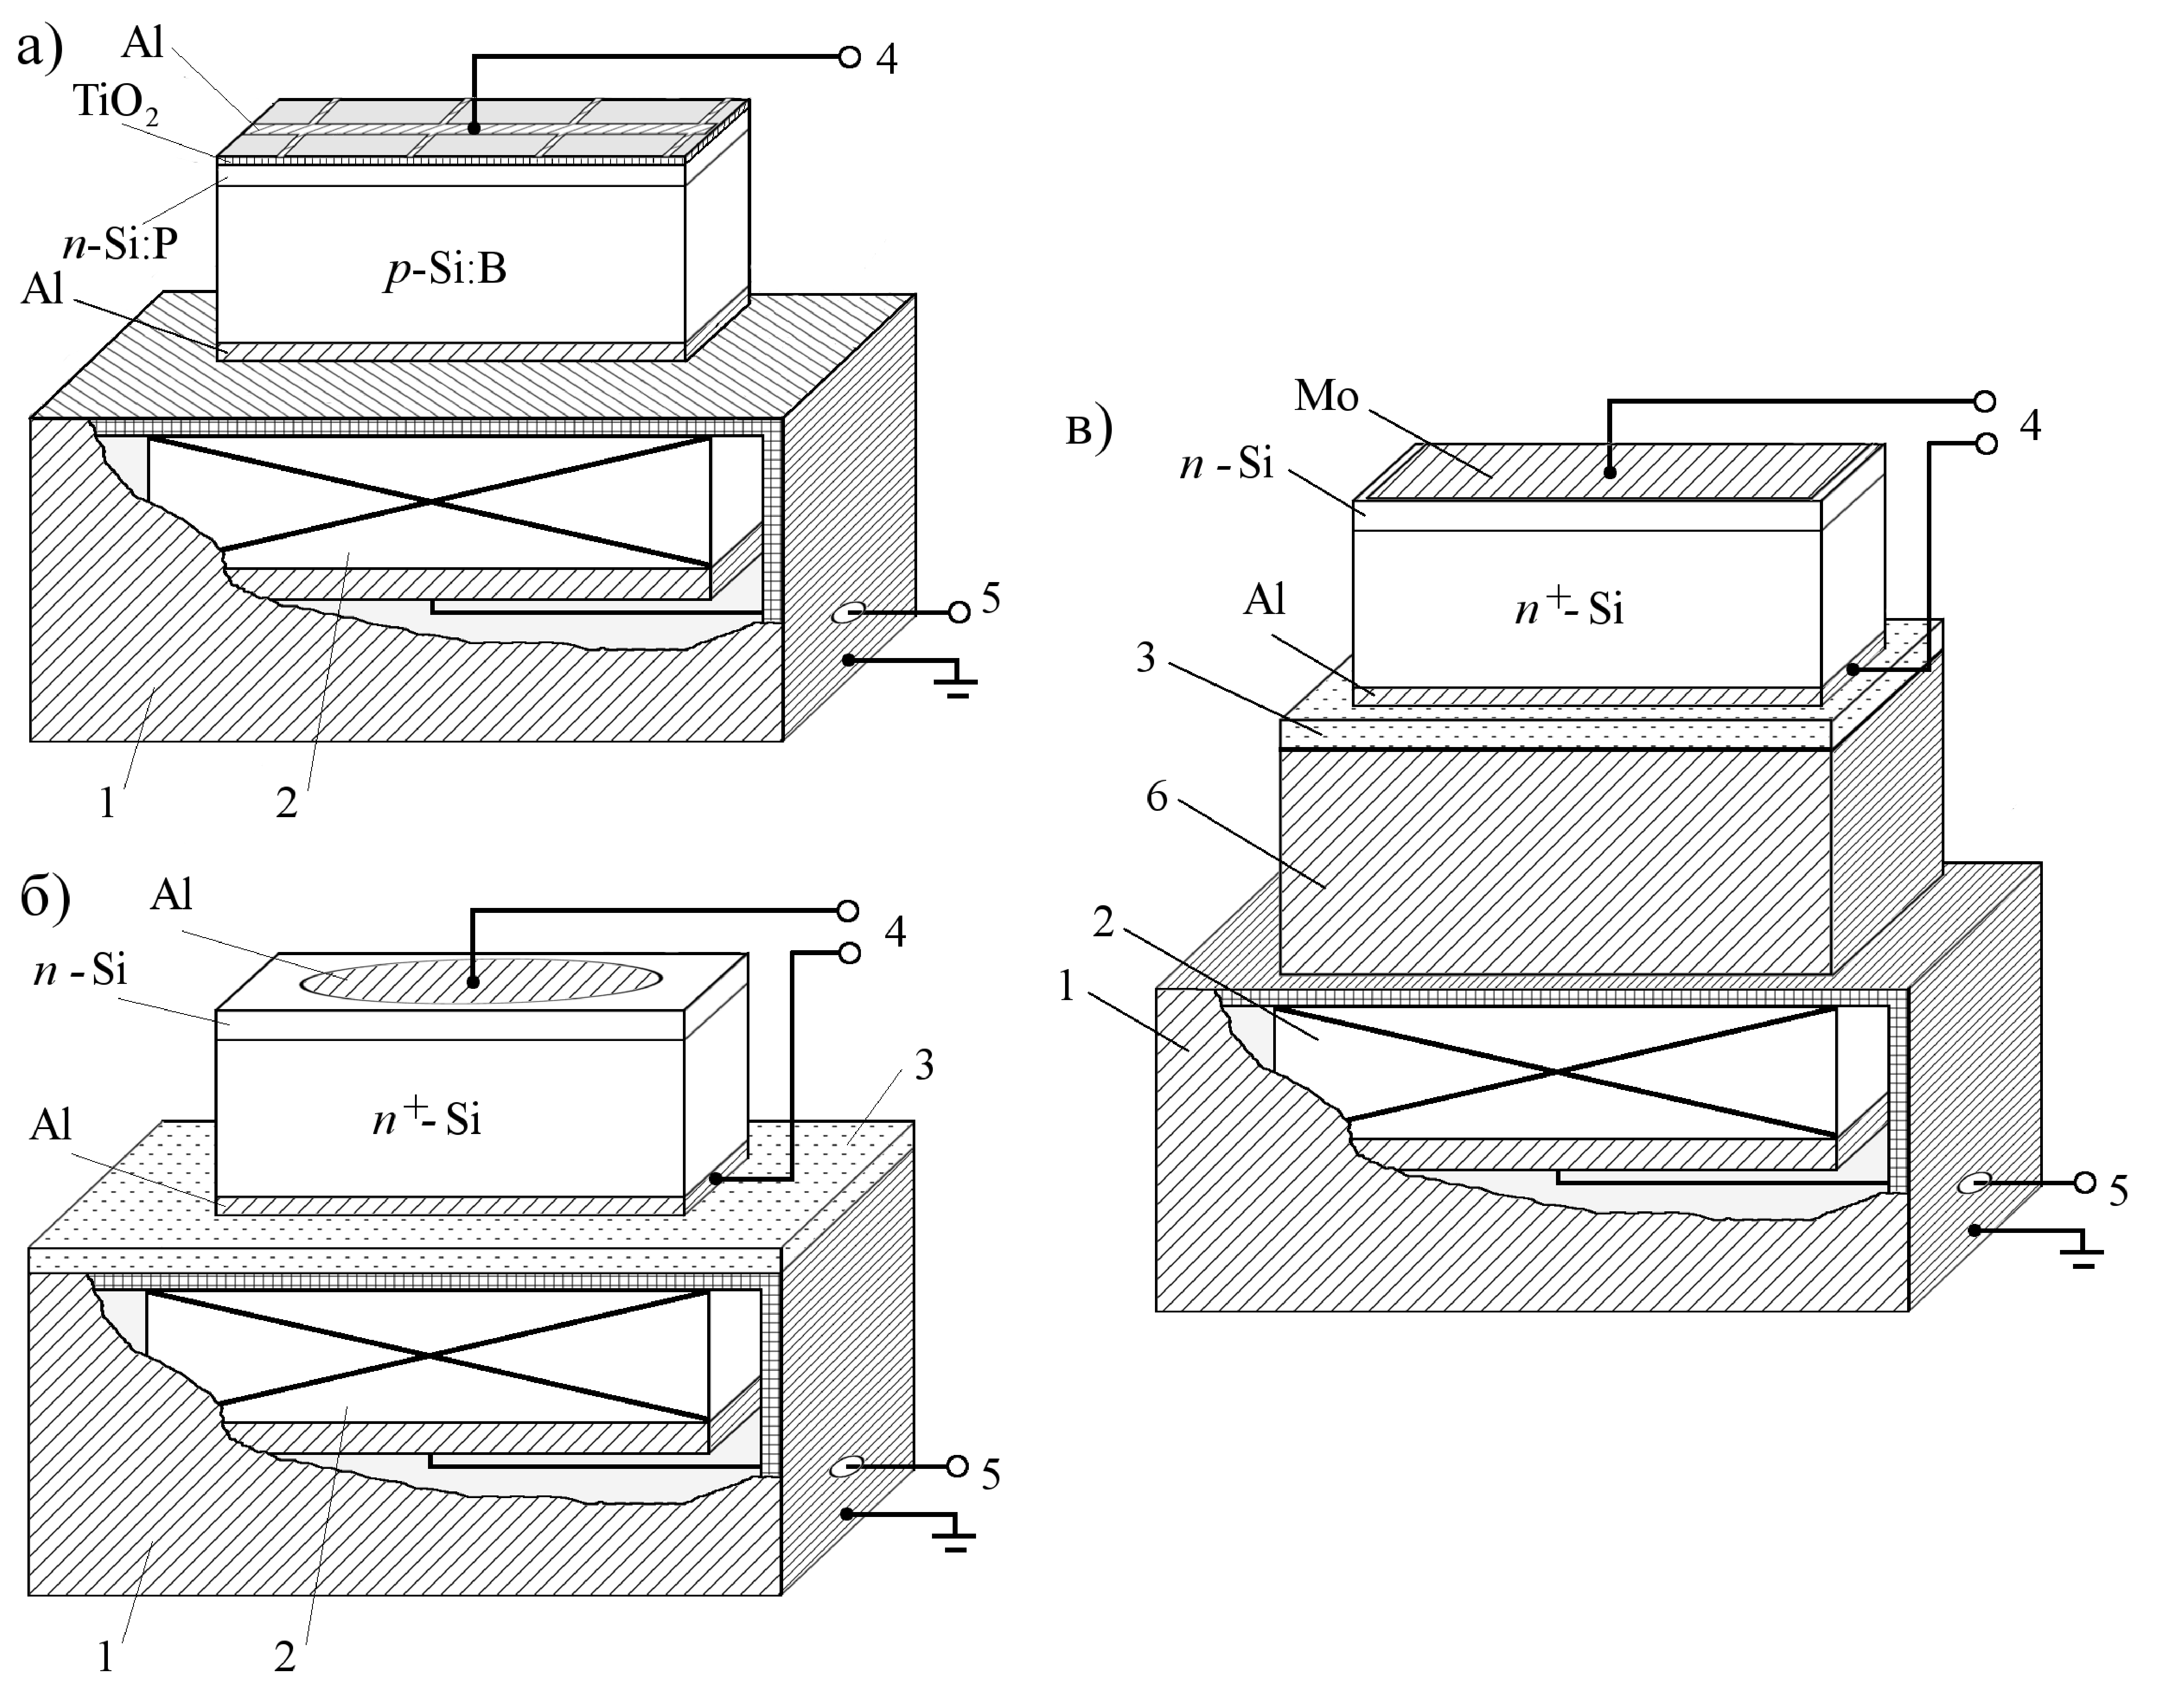
\includegraphics[width=1.0\textwidth]{USL}%
\caption{\label{figUSL}
Використані схеми УЗН кремнієвих структур: \protect\\
1 --  екран (алюмінієва фольга, товщина 0,012~мм);\protect\\
2 -- п'єзоелектричний перетворювач (LiNbO$_3$);\protect\\
3 -- діелектричний прошарок (слюда, товщина 0,03~мм);\protect\\
4 -- контакти для вимірювання вольт--амперних характеристик;\protect\\
5 -- контакти для збудження УЗ;\protect\\
6 -- буфер (алюмінієвий циліндр із високим ступенем паралельності граней, 2~см)
}
\end{figure}



Структури, в яких проводилися дослідження ефектів УЗН, містили енергетичний бар'єр, пов'язаний із наявністю контакту метал---напівпровідник або $p$---$n$--переходу, розміщений поблизу однієї з поверхонь зразка.
Введення УЗ відбувалось з боку грані, протилежної до місця розташування бар'єру.
 Напрям поширення АХ перпендикулярний площині бар'єру і збігається з напрямом струму, який виникає під час прикладення до структури електричної напруги (або при освітленні, якщо об'єктом дослідження є сонячний елемент).
  При використанні повздовжніх хвиль вимушені зміщення атомів відбуваються у тому самому напрямі, тоді як для поперечних хвиль коливання атомів спрямовані у площині бар'єру перпендикулярно до електричного струму .


Раніше показано \cite{Ostapenko1995,YOlikhTPL2011,Ostrovskii2001}, що характерний час зміни властивостей кремнієвих структур під дією УЗ не перевищує 2000~c.
З метою обмеження впливу будь--яких перехідних АІ процесів використовувалася наступна експериментально процедура.
УЗН починалося при кімнатній температурі.
Після цього зразки перебували не менше 60~хв за умов поширення в них пружних коливань і лише після цього, не припиняючи дії УЗ, починалися вимірювання електрофізичних параметрів та/або процеси нагріву або охолодження.


Відомо, що під час навантаження п'єзоелектричний перетворювач нагрівається.
Температура структур, які досліджувалися, контролювалася диференційною термопарою мідь--константан.
У роботі проводилось порівняння значень параметрів, отриманих за однакових температур в умовах УЗН зразків та без нього.
Це дозволяло виокремити АІ зміни характеристик напівпровідникових структур, від змін, пов'язаних із розігрівом зразків під час УЗН.
Для оцінки величини впливу УЗ на певний параметр $P$ (напруга холостого ходу, фактор неідеальності, величина зворотного струму тощо),
використовувалися абсолютні
$\Delta P$ чи відносні зміни $\varepsilon_P$
\begin{eqnarray}
  \label{eqAbsDelta} \Delta P &=& P_{in}-P_\mathtt{US}\,, \\
  \label{eqEpsDelta} \varepsilon_P &=& (P_{in}-P_\mathtt{US})/P_{in}\,,
\end{eqnarray}
% \begin{equation}
% \label{eqAbsDelta}
%\Delta P=P_{in}-P_\mathtt{US}\,,
% \end{equation}
%%чи відносні зміни
% \begin{equation}
% \label{eqEpsDelta}
%\varepsilon_P=\frac{P_{in}-P_\mathtt{US}}{P_{in}}\,,
% \end{equation}
де нижні індекси <<$\mathtt{US}$>> та <<$in$>> вказують на те, що відповідне значення параметра отримане при однаковій температурі за умов УЗН та без нього, відповідно.

При УЗО процеси впливу АХ та вимірювання параметрів розділені в часу і тому нагальної необхідності екранування п'єзоелектричних полів не було.
Як наслідок, експериментальна схема простіша, п'єзоперетворювач безпосередньо акустично контактував із досліджуваною структурою.


\subsection{Оцінка параметрів акустичного впливу\label{SC:USL}}
%\section{Режими ультразвукового навантаження кристалічних кремнієвих сонячних елементів\label{SC:USL}}


Для оцінки інтенсивності АХ, введеної у напівпровідникову структуру, використовувалася формула плоского п’єзоперетворювача \cite{WusBook}:
 \begin{equation}
 \label{eqWus}
 W_\mathtt{US}=4K_\mathtt{LNO}^2C_\mathtt{LNO}f_r\frac{\rho_\mathtt{LNO}\,\upsilon_\mathtt{LNO}}{\rho_\mathtt{Si}\,\upsilon_\mathtt{Si}}\frac{V_\mathtt{RF}^2}{A_\mathtt{LNO}M_0},
 \end{equation}
де
$K_\mathtt{LNO}$ --- коефіцієнт електромеханічного зв'язку,
$C_\mathtt{LNO}$ та $A_\mathtt{LNO}$ --- статична ємність закріпленого перетворювача та його площа, відповідно;
для використаних перетворювачів ємність складала 0,1$\div$0,3~нФ залежно від площі та товщини;
%$f_r$ --- резонансна частота;
$\rho_\mathtt{LNO}$ та $\rho_\mathtt{Si}$ --- густини LiNbO$_3$ та Si;
$\upsilon_\mathtt{LNO}$ та $\upsilon_\mathtt{Si}$ --- швидкості поширення звуку в LiNbO$_3$ та Si, відповідно;
$V_\mathtt{RF}$ --- амплітуда високочастотної напруги, прикладеної до перетворювача,
а коефіцієнт $M_0$ розраховується за допомогою співвідношення
 \begin{equation}
 \label{eqM0}
 M_0=\frac{\left[\cos\left(\pi\frac{f_\mathtt{US}}{f_r}\right)\right]^2+\left[\frac{\rho_\mathtt{LNO}\,\upsilon_\mathtt{LNO}}{\rho_\mathtt{Si}\,\upsilon_\mathtt{Si}}\sin\left(\pi\frac{f_\mathtt{US}}{f_r}\right)\right]^2}
 {\left[\sin\left(\frac{\pi}{2}\frac{f_\mathtt{US}}{f_r}\right)\right]^4}\,.
 \end{equation}
Відносна деформація при поширенні АХ описується виразом
 \begin{equation}
 \label{eqDefUS}
 \xi_{\mathtt{US}}=\sqrt{\frac{2W_\mathtt{US}}{\rho_\mathtt{Si}\,\upsilon_\mathtt{Si}^3}}\,,
 \end{equation}
тоді як амплітуда зміщень атомів
 \begin{equation}
 \label{eqAmpUS}
 u_{\mathtt{US}}=\sqrt{\frac{W_\mathtt{US}}{2\,\pi^2\,f_\mathtt{US}^2\,\rho_\mathtt{Si}\,\upsilon_\mathtt{Si}}}\,.
 \end{equation}

Параметри, які використовувалися при розрахунках, наведено в табл.~\ref{tabLNO}.


\begin{table}
\caption{\label{tabLNO}Окремі параметри LiNbO$_3$ та Si при кімнатній температурі \cite{WusBook,ShackBook}
}
%\begin{tabular}{|l|l|c|}
%\begin{tabularx}{\textwidth}{|>{\raggedright\arraybackslash}X|>{\centering\arraybackslash}X|>{\centering\arraybackslash}X|}
\begin{tabularx}{\textwidth}{|l|>{\centering\arraybackslash}X|>{\centering\arraybackslash}X|}
\hline
$K_\mathtt{LNO}^2$&зріз $(Y\!+\!36^\circ)$&0,24\\
\cline{2-3}
&зріз $(Y\!+\!163^\circ)$&0,46\\
\hline
$\upsilon_\mathtt{LNO}$,&повздовжні хвилі&7340\\
\cline{2-3}
м/с&поперечні хвилі&4560\\
\hline
&повздовжні хвилі, $[100]$&8430\\
\cline{2-3}
&повздовжні хвилі, $[111]$&9850\\
\cline{2-3}
$\upsilon_\mathtt{Si}$,&повздовжні хвилі, $[110]$&9130\\
\cline{2-3}
м/с&поперечні хвилі, $[110]\,/\,[1\bar{1}0]$&4670\\
\cline{2-3}
&поперечні хвилі, $[110]\,/\,[001]$&5840\\
\cline{2-3}
&поперечні хвилі, $[111]\,/\,$довіл.&5090\\
\hline
\multicolumn{2}{|l|}{$\rho_\mathtt{LNO}$, кг/м$^3$}&4700\\
\hline
\multicolumn{2}{|l|}{$\rho_\mathtt{Si}$, кг/м$^3$}&2328\\
\hline
%\end{tabular}
\end{tabularx}
\end{table}

Дослідження, результати яких наведено в розділах~\ref{Ch_SSC}, \ref{Ch_GammaSD} та \ref{Ch_UST_MW},  проводились у достатньо вузькому температурному діапазоні $290\div340$~К.
При цьому вважалось, що параметри п'зоелектричного перетворювача змінюються мало, сталість величини $V_\mathtt{RF}$ забезпечує незмінність $W_\mathtt{US}$  для всього діапазону температур.
Вплив екрануючого прошарку на інтенсивність звуку, введеного в зразок, вважався знехтувано малим, оскільки його товщина значно менша ніж половина довжини АХ.

\subsection{Особливості низькотемпературного ультразвукового \mbox{навантаження}\label{SSDB:USL}}

Ультразвукове навантаження структур Mo---$n$--$n^+$--Si (розділ~\ref{Ch_USL_T_SD}) здійснювалося в діапазоні температур 130$\div$330~К за схемою, наведеною на рис.~\ref{figUSL},в.
У випадку низькотемпературного (при $T<230$~К) УЗН процес збудження АХ був ускладнений через те, що
рідкі акустичні склейки на кшталт вакуумного масла кристалізувалися і переставали виконувати свою функцію.
Водночас, контакт створений при кімнатній температурі за допомогою жорсткої склейки (піцеїн або БФ6),
руйнувався при охолодженні внаслідок різниці коефіцієнтів теплового розширення.
У роботі низькотемпературне УЗН (повздовжні хвилі) здійснювалося за допомогою свіжого (до 5~год після нанесення) контакту з клею БФ6,
який ще не повністю кристалізувався.
Наявність акустичного контакту контролювалася за виглядом залежності повного опору перетворювача від частоти,
де за наявності акустичного контакту з'являвся ряд максимумів, пов'язаних із відбиванням хвиль від граней буфера.

\begin{figure}
\center
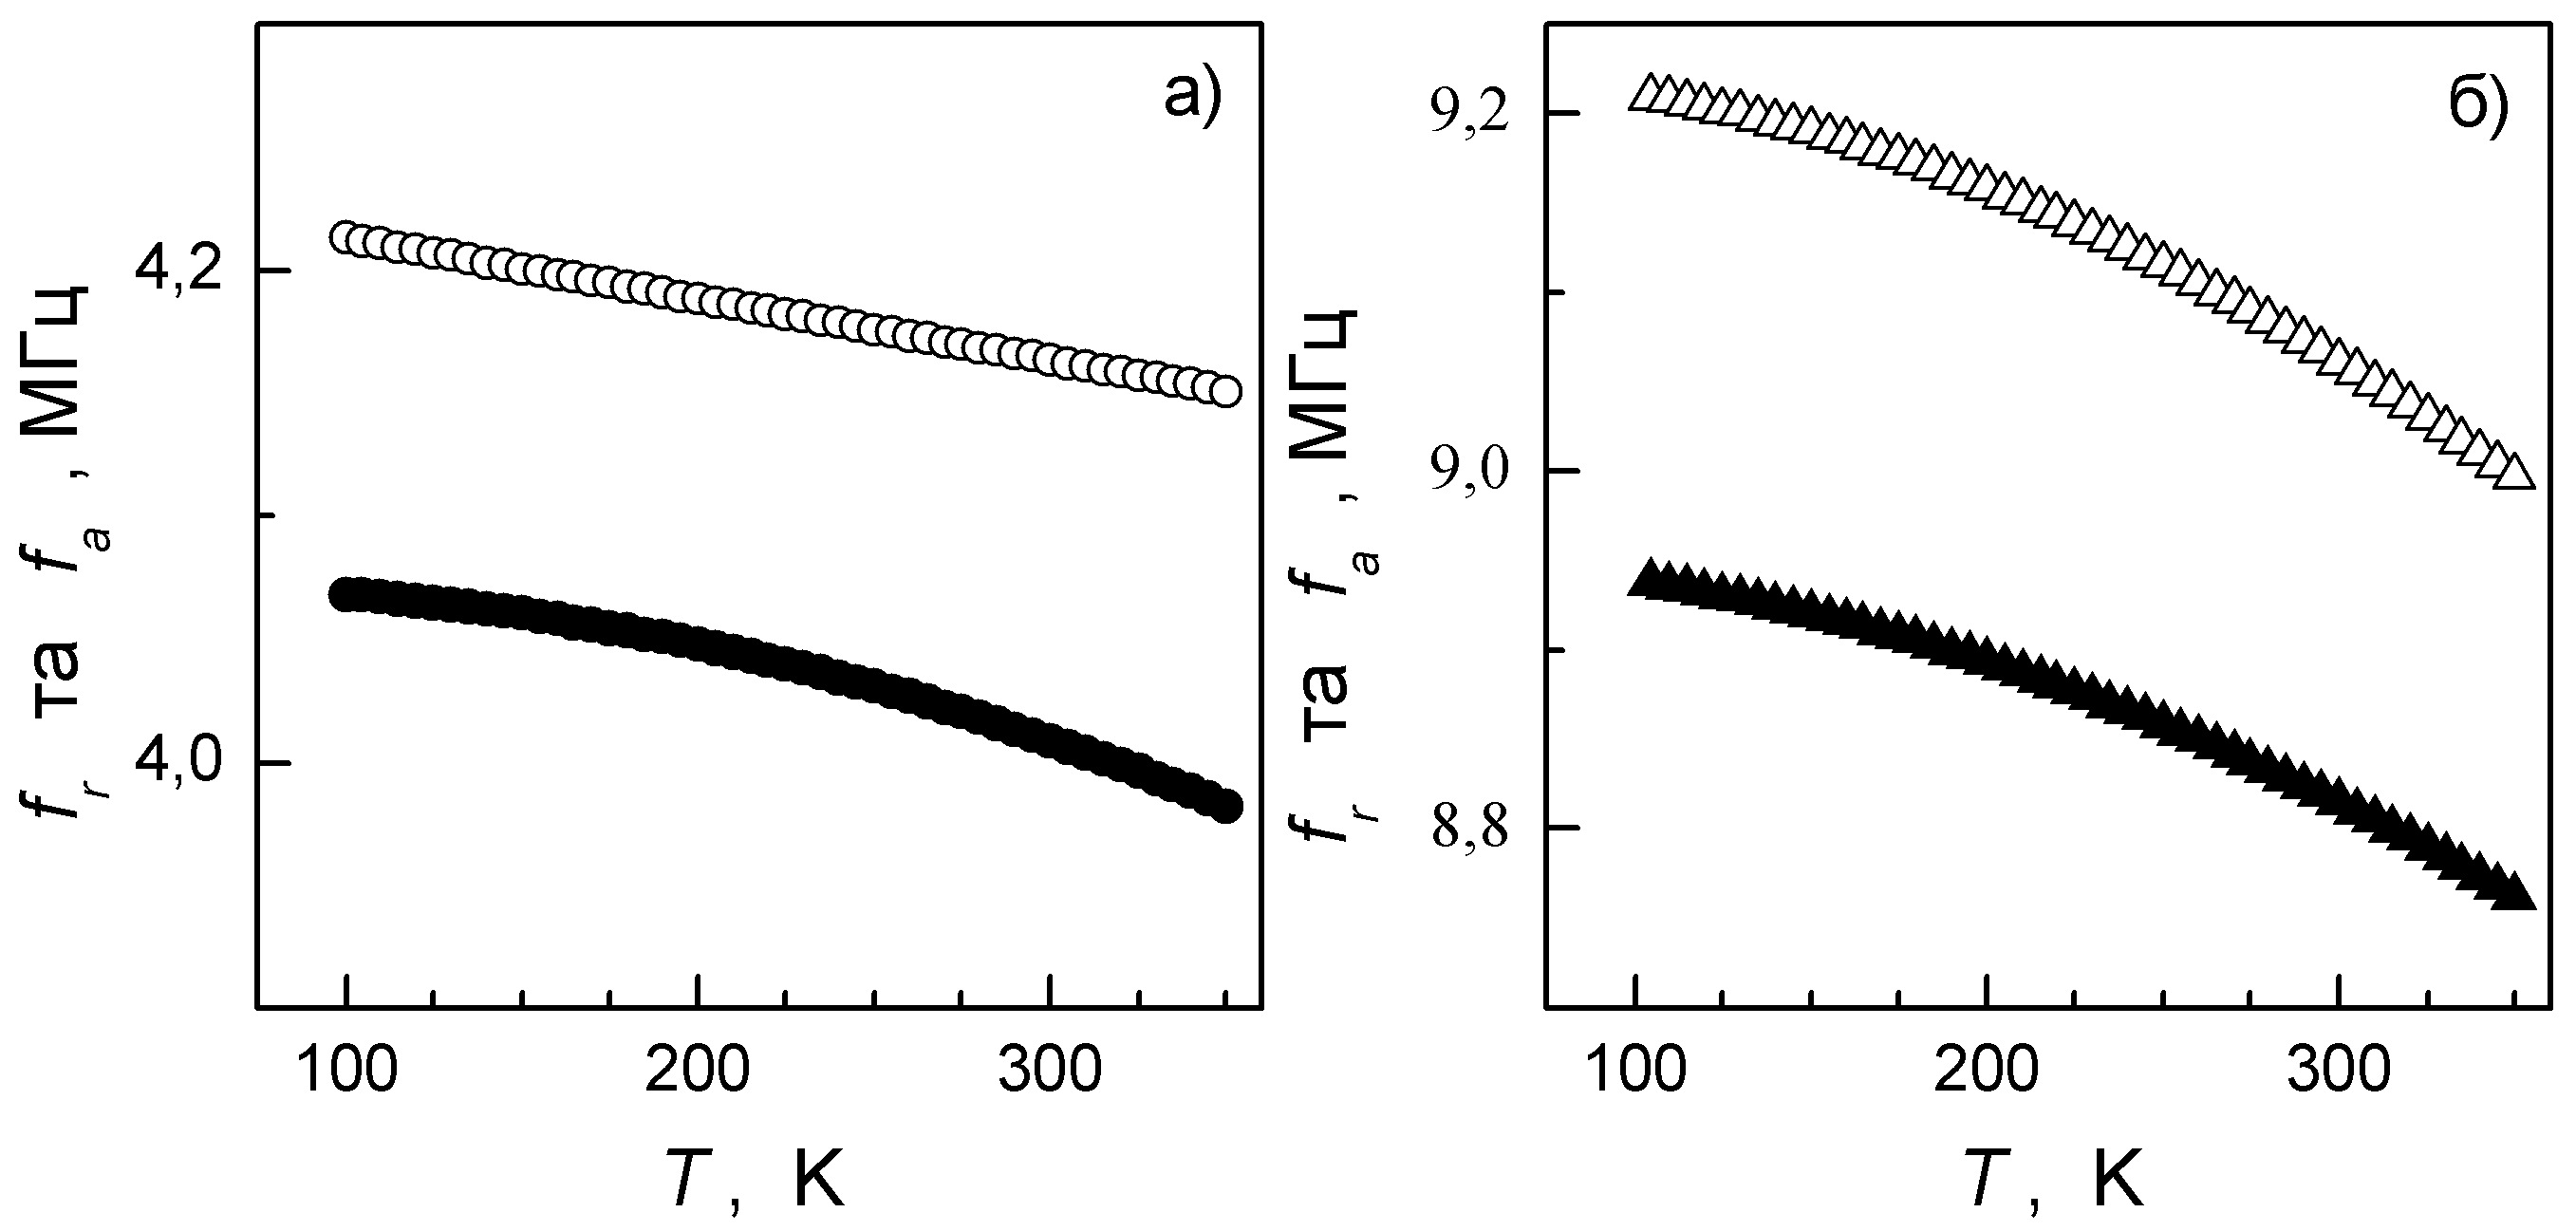
\includegraphics[width=0.8\textwidth]{figFrT}%
\caption{\label{figFrT}
Температурна залежність частот резонансу (заповнені точки) та антирезонансу (порожні точки) (перша гармоніка)
п'єзоелектричних перетворювачів LiNbO$_3$ з робочими частотами $f_\mathtt{US}$ 4,1~МГц (а) та 9,6 (б)~МГц при кімнатній температурі
}
\end{figure}


Водночас при визначенні параметрів УЗН за допомогою формул (\labelcref{eqAmpUS,eqWus,eqM0,eqDefUS}) та даних табл.~\ref{tabLNO} викликає ряд труднощів.
По--перше, параметри матеріалу є температурозалежними.
Наприклад, із літератури відомо, що зміна пружних сталих при збільшенні температури на 100 К для LiNbO$_3$ становить приблизно (-2\%) \cite{LNO_C:Temp},
а для кремнію --- (-2.5\%) \cite{Si_C:Temp};
типові температурні залежності резонансної та антирезонансної частот показані на рис.~\ref{figFrT}.
Широкий температурний інтервал дослідження АІ ефектів не дозволяв нехтувати подібними залежностями.
%При дослідженні АІ ефектів в структурах SSDB вимірювання проводилися в достатньо широкому температурному інтервалі і тому подібними залежностями нехтувати не можна.
По--друге, наявність буфера спричинювала втрати акустичної енергії внаслідок поглинання УЗ в алюмінієвому циліндрі, часткового відбивання пружних хвиль
при переході з одного середовища в інше тощо.
Ці ефекти також не враховані у виразах (\ref{eqWus}) і  (\ref{eqM0}).
Відтак, оцінка інтенсивності введеного УЗ здійснювалася за допомогою виразу
 \begin{equation}
 \label{eqWus2}
 W_\mathtt{US}=\frac{V_\mathtt{RF}^2}{2\,A_\mathtt{LNO}\,Z_\mathtt{LNO}}\,K_\mathtt{LNO}^2\,l_\mathtt{US},
 \end{equation}
де
$Z_\mathtt{LNO}$ --- імпеданс акустично навантаженого перетворювача,
$l_\mathtt{US}$ --- коефіцієнт, який враховує загальні втрати пружної енергії.
При цьому вважалося, що величини
$K_\mathtt{LNO}$, $Z_\mathtt{LNO}$ та $l_\mathtt{US}$ залежать від температури.

Визначення $K_\mathtt{LNO}$ та $l_\mathtt{US}$ відбувалося з використанням стандартної схеми,
зображеної на рис.~\ref{Luna2},а.
У системі збуджувалися імпульси УЗ за допомогою одного з ідентичних п'єзоперетворювачів і реєструвалися
високочастотні сигнали на другому.
Амплітуди сигналів $V_\mathtt{RF}^{(1)}$ та $V_\mathtt{RF}^{(2)}$, пов'язаних із однократним та троєкратний (після відбиття від правої та лівої меж) проходженням акустичного імпульсу через систему
(рис.~\ref{Luna2},б) можуть бути записані у вигляді
\begin{eqnarray}
  \label{eqVrf1} (V_\mathtt{RF}^{(1)})^2&=&V_\mathtt{RF}^2\,K_\mathtt{LNO}^4\,l_\mathtt{US}, \\
  \label{eqVrf2} (V_\mathtt{RF}^{(2)})^2&=&V_\mathtt{RF}^2\,K_\mathtt{LNO}^4\,l_\mathtt{US}^3.
\end{eqnarray}

% \begin{equation}
% \label{eqVrf1}
% (V_\mathtt{RF}^{(1)})^2=V_\mathtt{RF}^2\,K_\mathtt{LNO}^4\,l_\mathtt{US},
% \end{equation}
% \begin{equation}
% \label{eqVrf2}
% (V_\mathtt{RF}^{(2)})^2=V_\mathtt{RF}^2\,K_\mathtt{LNO}^4\,l_\mathtt{US}^3.
% \end{equation}

\begin{figure}
\center
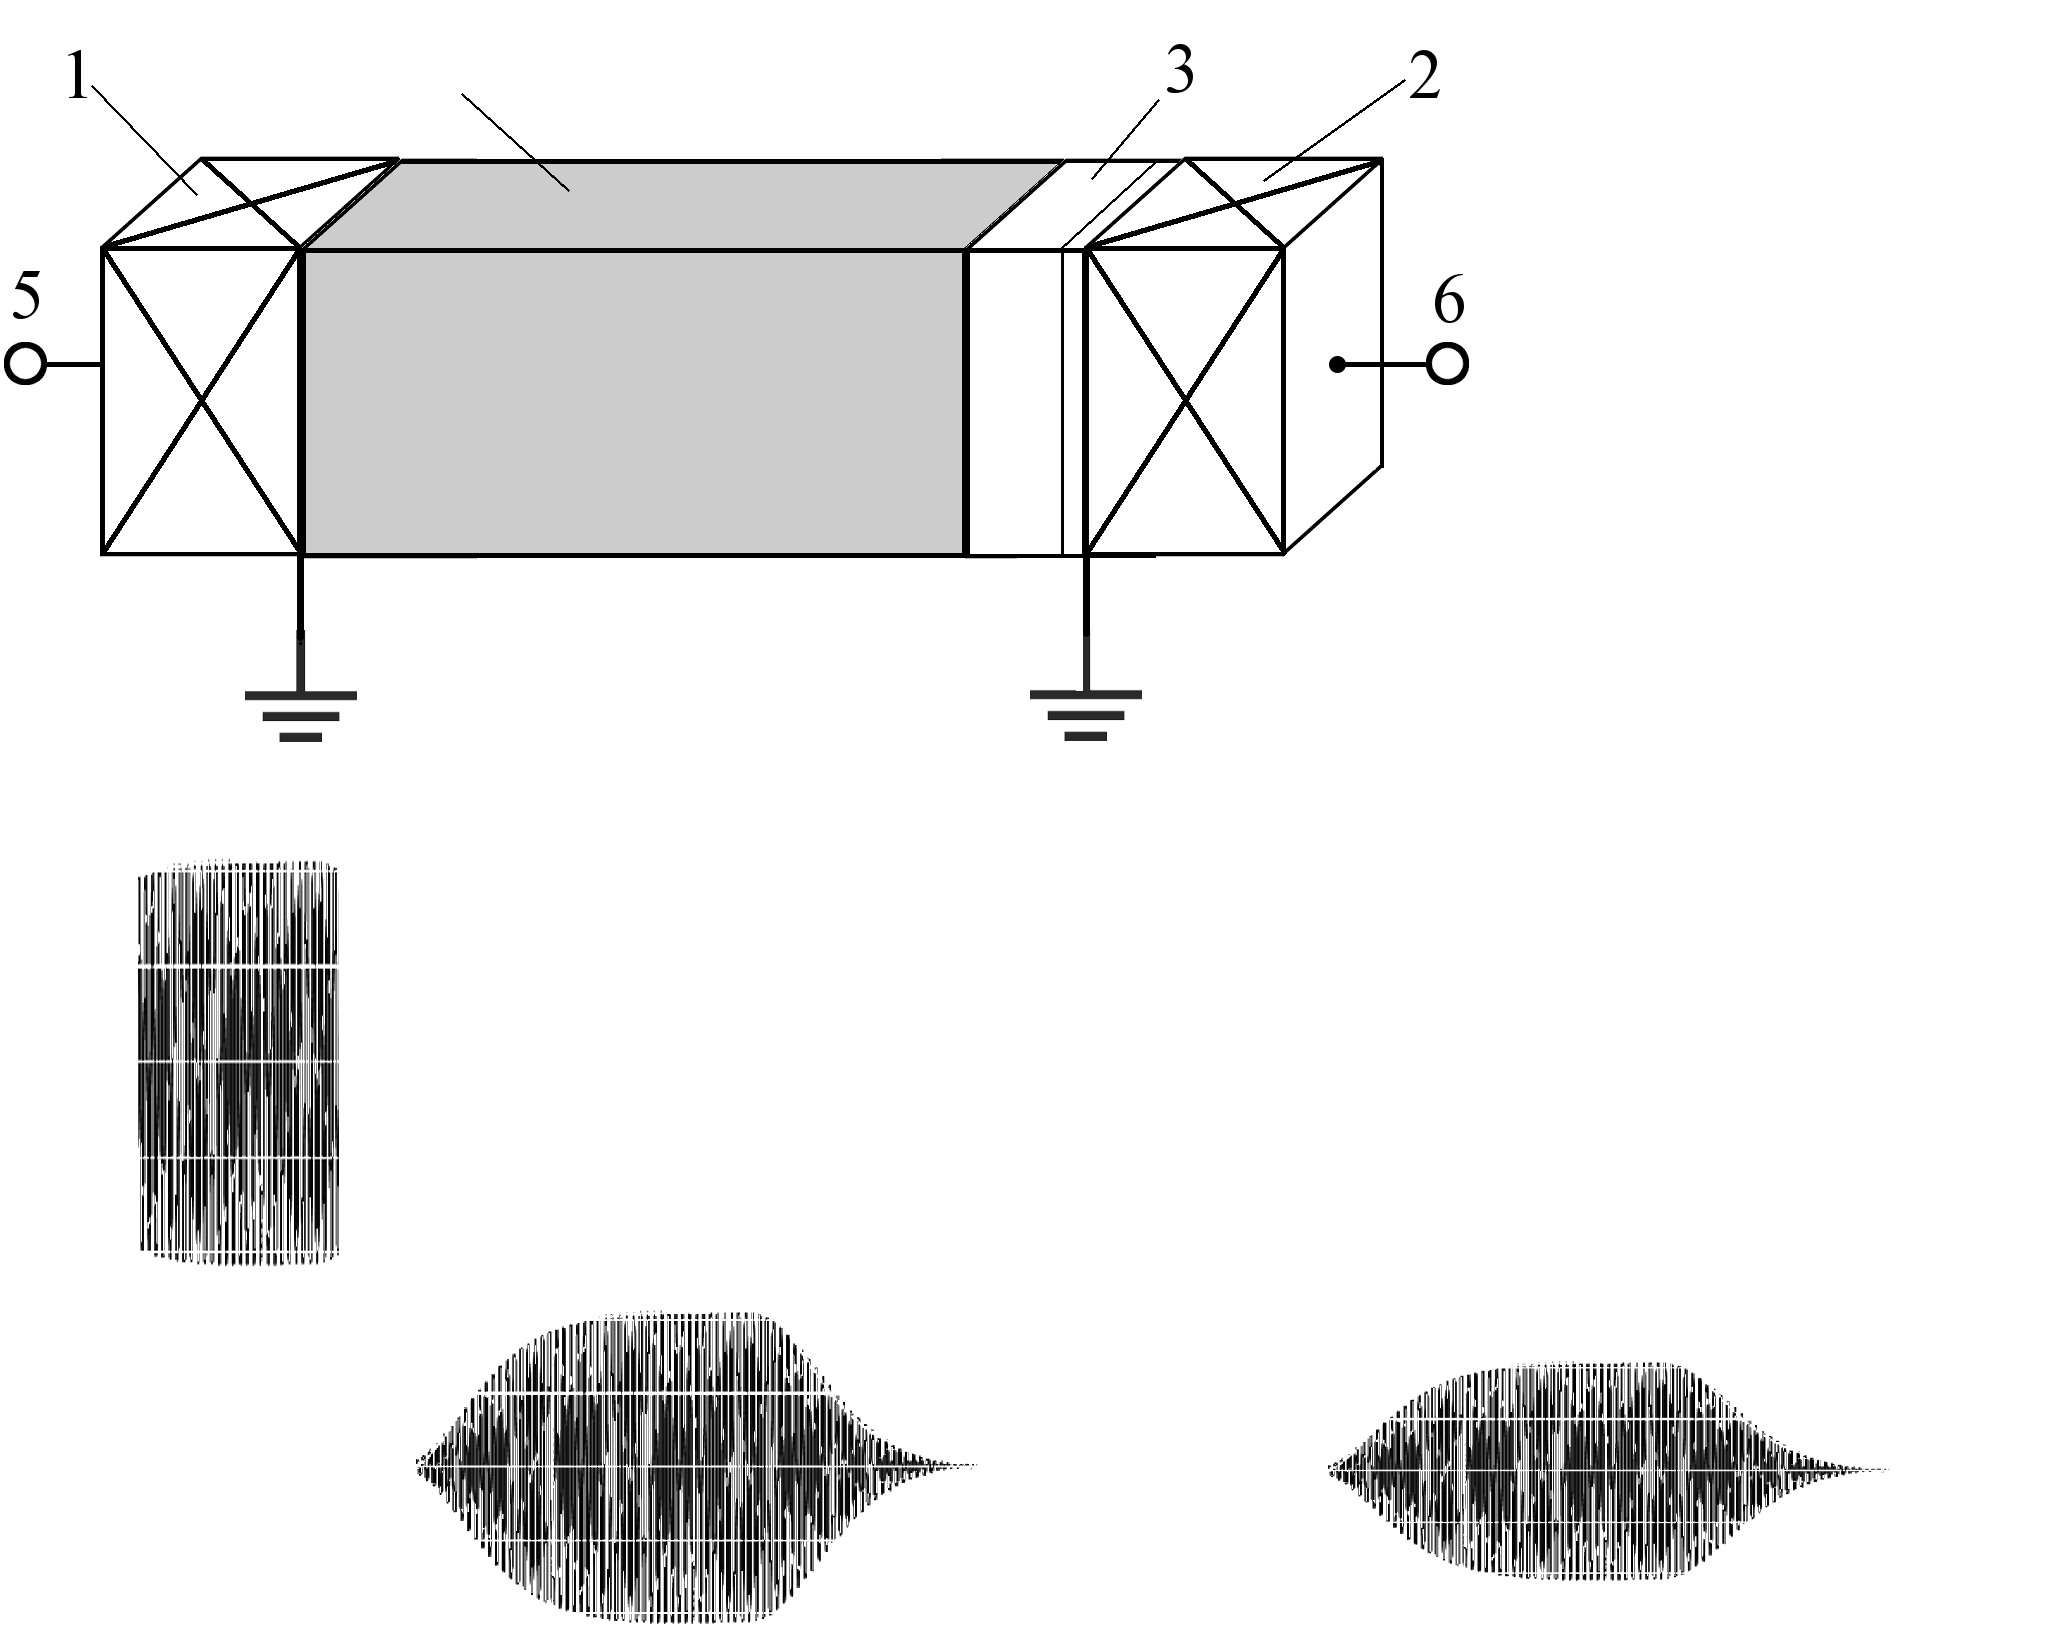
\includegraphics[width=0.9\textwidth]{Luna2}%
\caption{\label{Luna2}
а) Схема для оцінки інтенсивності введеного УЗ:\protect\\
1, 2 -- ідентичні п'єзоелектричні перетворювачі; \protect\\
3 -- напівпровідникова структура;\protect\\
4 -- буфер; \protect\\
5, 6 --- електроди збуджуючого та приймаючого перетворювачів, відповідно. \protect\\
б) Схематична осцилограма сигналів на електродах п'єзоперетворювачів. \protect\\
в) Схема для визначення імпедансу п'єзоперетворювача: \protect\\
7 -- датчик струму; \protect\\
8 -- еталонний опір
}
\end{figure}

Останні два співвідношення дозволяють визначити акустичні параметри системи на основі вимірювання амплітуд
високочастотних сигналів на електродах збуджуючого та приймаючого п'єзоперетворювачів.
Приклад отриманих температурних залежностей наведено на рис.~\ref{figKp2T}.

\begin{figure}
\center
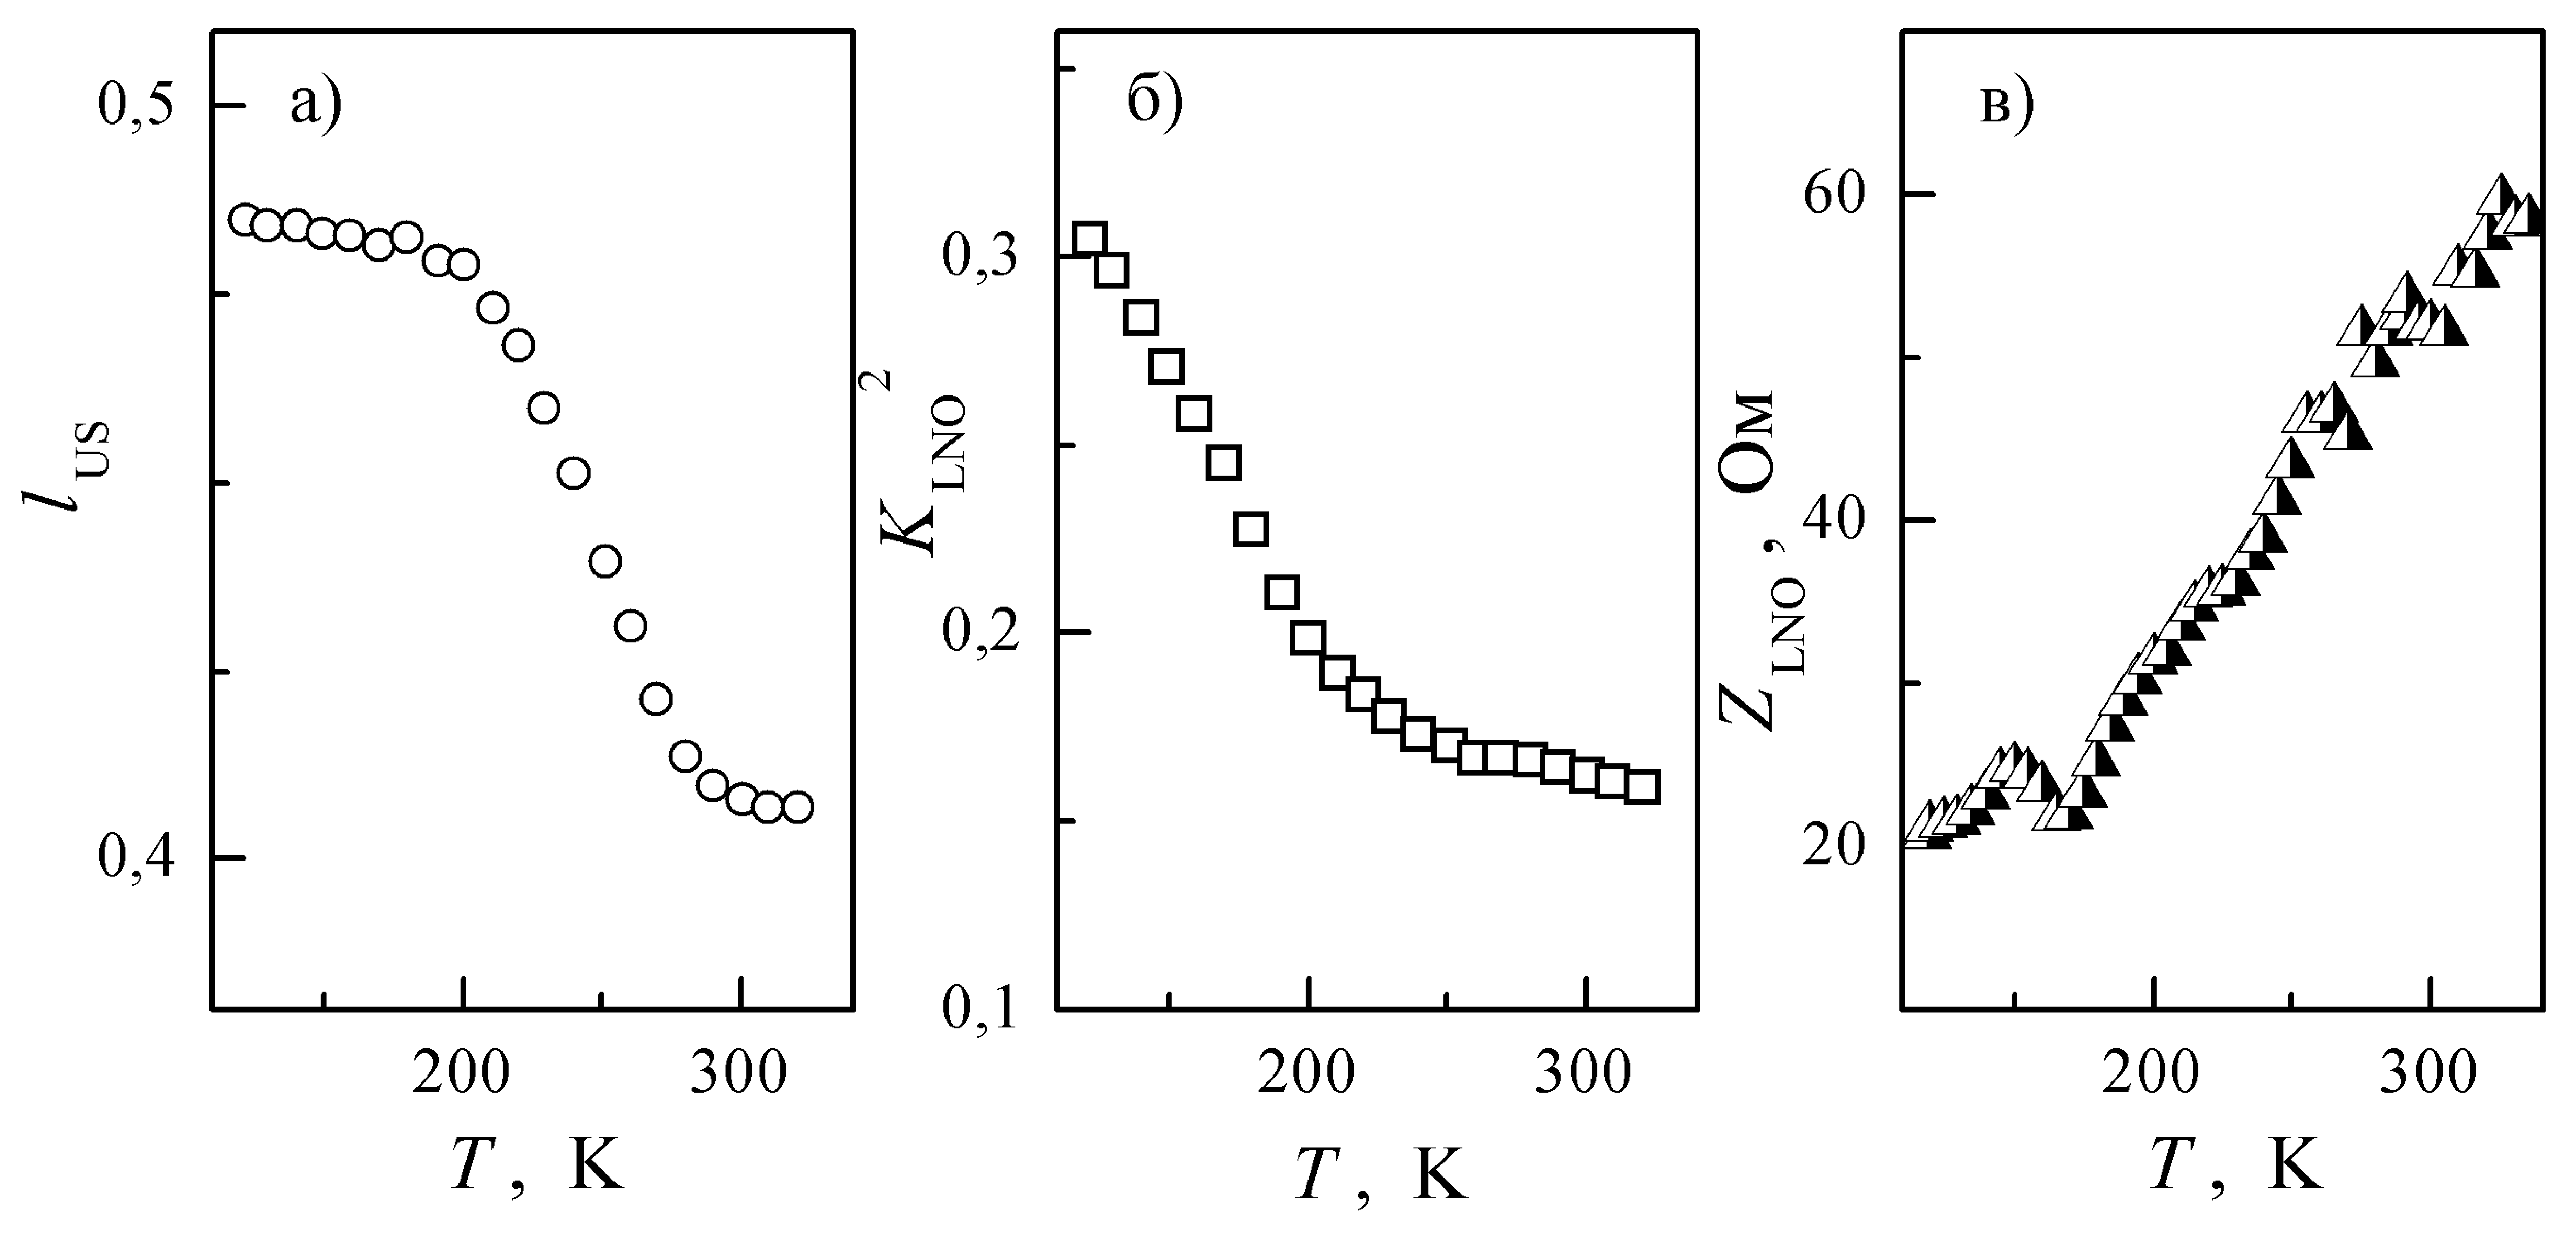
\includegraphics[width=0.9\textwidth]{figKp2T}%
\caption{\label{figKp2T}
Температурні залежності коефіцієнта акустичних втрат (а),
квадрата коефіцієнта електромеханічного зв'язку (б) та
імпедансу (в) п'єзоперетворювача з робочою частотою $f_\mathtt{US}=8,4$~МГц}
\end{figure}

Для оцінки $Z_\mathtt{LNO}$ використовувався метод,
схема якого представлена на рис.~\ref{Luna2},в.
Датчиком струму слугувало феритове кільце із дротяною обмоткою.
Кількість витків обмотки підбиралось для кожної частоти таким чином, щоб для випадку, коли під'єднано еталонний опір $R_\mathtt{st}$,
зсув фаз між збуджуючим сигналом амплітудою $V_\mathtt{RF,st}$ та сигналом із датчика амплітудою $V_\mathtt{L,st}$
дорівнював нулеві.
Величина імпедансу розраховувалася за допомогою виразу
 \begin{equation}
 \label{eqZlno}
 Z_\mathtt{LNO}=\frac{V_\mathtt{RF}}{V_\mathtt{L}}\,\frac{V_\mathtt{L,st}}{V_\mathtt{RF,st}}\,R_\mathtt{st}.
 \end{equation}

У роботі використовувався еталонний опір величиною 56,7~Ом.
Температурна залежність імпедансу одного з перетворювачів наведена на рис.~\ref{figKp2T},в.

Використання виразу (\ref{eqWus2}) та даних рис.~\ref{figKp2T} показує, що при подачі на електроди п'єзоелектричного перетворювача
високочастотної напруги з постійною амплітудою в діапазоні температур 130$\div$330~K призводить до поширення у зразку АХ з
інтенсивністю, яка змінюється більше ніж в п'ять разів --- рис.~\ref{figWusT},а.
З іншого боку, поблизу кімнатних температур наближення попереднього пункту, яке стосується незмінності значення $ W_\mathtt{US}$
при постійній величині $V_\mathtt{RF}$, справедливе з точністю до 10 відсотків.
На рис.~\ref{figWusT},б також показано як має змінюватись амплітуда напруги на п'єзоперетворювачі, щоб при різних температурах
інтенсивність УЗН залишалась постійною.


\begin{figure}
\center
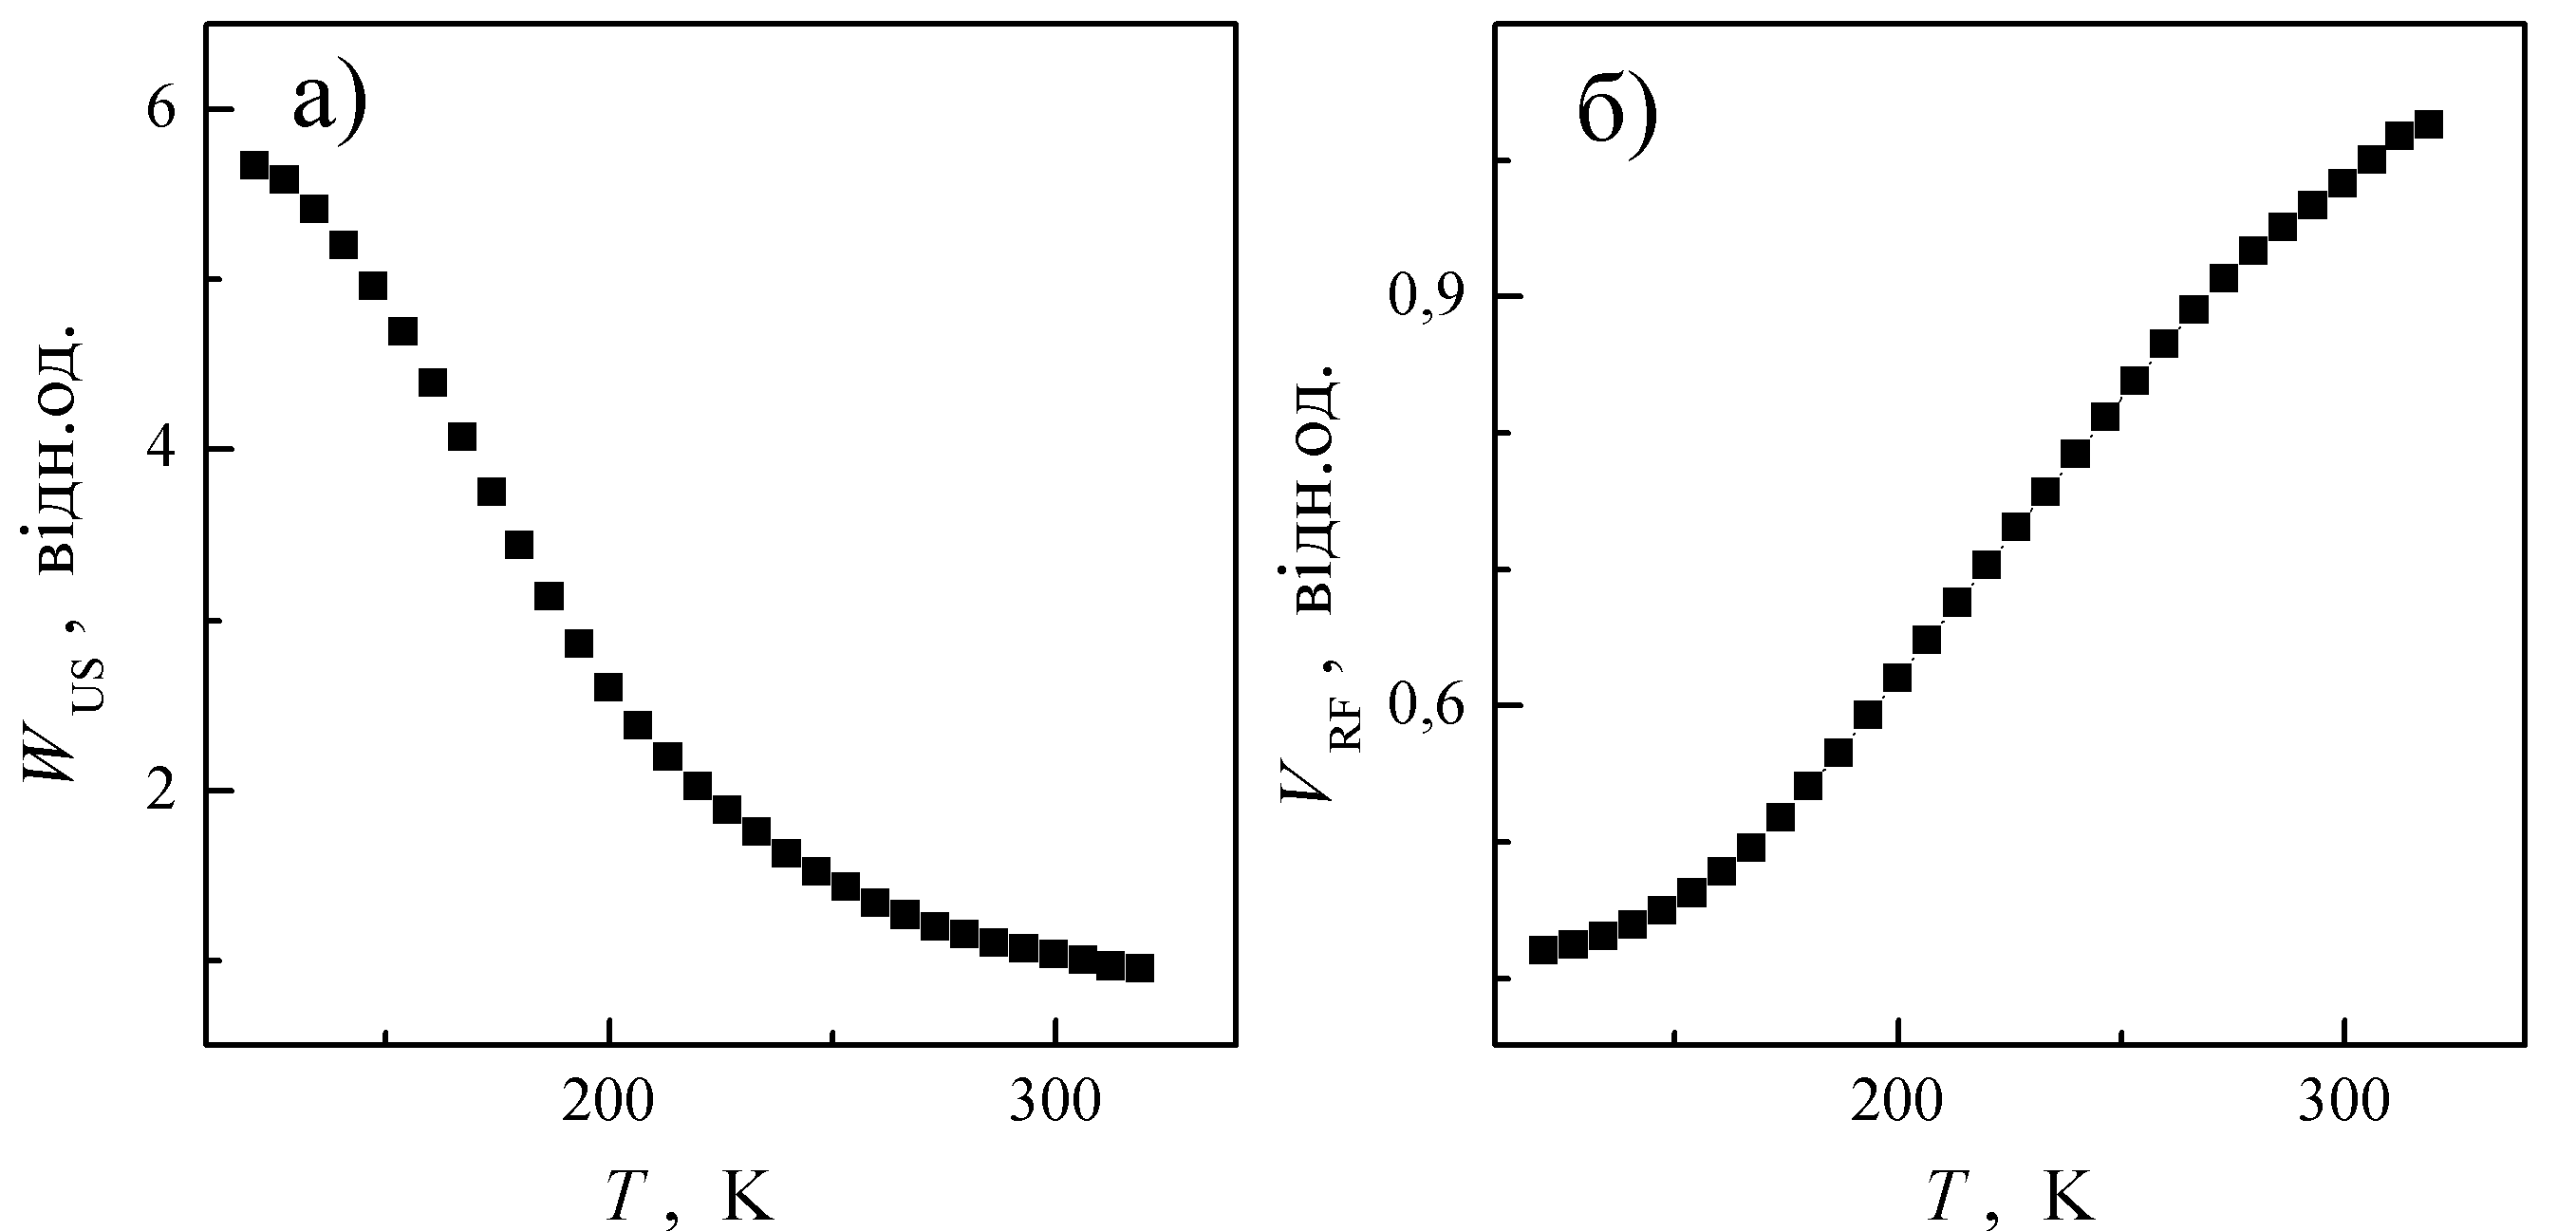
\includegraphics[width=0.8\textwidth]{figWusT}%
\caption{\label{figWusT}
Температурні залежності
інтенсивності введеного УЗ при постійному значенні амплітуди напруги на п'єзоперетворювачі (а)
та необхідної амплітуди на п'єзоперетворювачі для постійності інтенсивності введеного УЗ (б)
для п'єзоперетворювача з робочою частотою $f_\mathtt{US}=8,4$~МГц.
}
\end{figure}




